%%%%%%%%%%%%%%%%%%%%%%%%%%%%%%%%%%%%%%%%%
% Masters/Doctoral Thesis
% LaTeX Template
% Version 2.3 (25/3/16)
%
% This template has been downloaded from:
% http://www.LaTeXTemplates.com
%
% Version 2.x major modifications by:
% Vel (vel@latextemplates.com)
%
% This template is based on a template by:
% Steve Gunn (http://users.ecs.soton.ac.uk/srg/softwaretools/document/templates/)
% Sunil Patel (http://www.sunilpatel.co.uk/thesis-template/)
%
% Template license:
% CC BY-NC-SA 3.0 (http://creativecommons.org/licenses/by-nc-sa/3.0/)
%
%%%%%%%%%%%%%%%%%%%%%%%%%%%%%%%%%%%%%%%%%

%----------------------------------------------------------------------------------------
%	PACKAGES AND OTHER DOCUMENT CONFIGURATIONS
%----------------------------------------------------------------------------------------

\documentclass[
captions=nooneline,
11pt, % The default document font size, options: 10pt, 11pt, 12pt
%oneside, % Two side (alternating margins) for binding by default, uncomment to switch to one side
%chapterinoneline,% Have the chapter title next to the number in one single line
ngerman, % ngerman for German
singlespacing, % Single line spacing, alternatives: onehalfspacing or doublespacing
%draft, % Uncomment to enable draft mode (no pictures, no links, overfull hboxes indicated)
%nolistspacing, % If the document is onehalfspacing or doublespacing, uncomment this to set spacing in lists to single
%liststotoc, % Uncomment to add the list of figures/tables/etc to the table of contents
%toctotoc, % Uncomment to add the main table of contents to the table of contents
%parskip, % Uncomment to add space between paragraphs
%nohyperref, % Uncomment to not load the hyperref package
headsepline, % Uncomment to get a line under the header
]{MastersDoctoralThesis} % The class file specifying the document structure

\usepackage[utf8]{inputenc} % Required for inputting international characters
\usepackage[T1]{fontenc} % Output font encoding for international characters
\usepackage{amsmath}
\usepackage{amssymb}
\usepackage{palatino} % Use the Palatino font by default
\usepackage{lscape}
\usepackage[]{algorithm2e}
\usepackage{caption}
\usepackage{fancyvrb}
\usepackage{multirow}
\usepackage{graphics}
\usepackage{rotating}
\usepackage{multicol}
\usepackage{mathtools}
\usepackage{chngcntr}
\usepackage{adjustbox}
\usepackage{bbm}
\usepackage{romannum}
\usepackage[usenames,dvipsnames,svgnames,table]{xcolor}

\renewcommand*\rmdefault{bch} % bch

\PassOptionsToPackage{hyphens}{url}\usepackage{hyperref}
\hypersetup{
     colorlinks   = true,
     citecolor    = gray,
     linkcolor    = blue
}

\VerbatimFootnotes
\captionsetup{margin=10pt,font=small,labelfont=bf}

\usepackage[backend=bibtex,style=authoryear,natbib=true]{biblatex} % Use the bibtex backend with the authoryear citation style (which resembles APA)

\addbibresource{example.bib} % The filename of the bibliography
\DefineBibliographyStrings{ngerman}{
   andothers = {{et\,al\adddot}},
}

\counterwithout{footnote}{chapter}

\usepackage[autostyle=true]{csquotes} % Required to generate language-dependent quotes in the bibliography

\newenvironment{itquote}
  {\begin{quote}\itshape}
  {\end{quote}\ignorespacesafterend}

\DeclareUnicodeCharacter{00A0}{ }

\makeatletter
\newcommand{\vast}{\bBigg@{4}}
\newcommand{\Vast}{\bBigg@{5}}
\makeatother

\DeclarePairedDelimiter\floor{\lfloor}{\rfloor}

%----------------------------------------------------------------------------------------
%	MARGIN SETTINGS
%----------------------------------------------------------------------------------------

\geometry{
	paper=a4paper, % Change to letterpaper for US letter
	inner=2.5cm, % Inner margin
	outer=3.8cm, % Outer margin
	bindingoffset=2cm, % Binding offset
	top=1.5cm, % Top margin
	bottom=1.5cm, % Bottom margin
	%showframe,% show how the type block is set on the page
}

\DeclareSymbolFont{extraup}{U}{zavm}{m}{n}
\DeclareMathSymbol{\varheart}{\mathalpha}{extraup}{86}

\def\changemargin#1#2{\list{}{\rightmargin#2\leftmargin#1}\item[]}
\let\endchangemargin=\endlist

%----------------------------------------------------------------------------------------
%	THESIS INFORMATION
%----------------------------------------------------------------------------------------

\thesistitle{Analyse der Relationsvorhersage im Deutschen mithilfe von Wortvektorrepräsentationen} % Your thesis title, this is used in the title and abstract, print it elsewhere with \ttitle
\thesistitleenglish{Analysis of relation prediction in German using word vector representations}
\supervisor{Dr. Yannick \textsc{Versley}} % Your supervisor's name, this is used in the title page, print it elsewhere with \supname
\examiner{} % Your examiner's name, this is not currently used anywhere in the template, print it elsewhere with \examname
\degree{Bachelor of Arts} % Your degree name, this is used in the title page and abstract, print it elsewhere with \degreename
\author{Dennis \textsc{Ulmer}} % Your name, this is used in the title page and abstract, print it elsewhere with \authorname
\addresses{} % Your address, this is not currently used anywhere in the template, print it elsewhere with \addressname

\subject{Computerlinguistik} % Your subject area, this is not currently used anywhere in the template, print it elsewhere with \subjectname
\keywords{} % Keywords for your thesis, this is not currently used anywhere in the template, print it elsewhere with \keywordnames
\university{Ruprecht-Karls-Universität Heidelberg} % Your university's name and URL, this is used in the title page and abstract, print it elsewhere with \univname
\universityenglish{Ruprecht-Karls University Heidelberg}
\department{Institut für Computerlinguistik} % Your department's name and URL, this is used in the title page and abstract, print it elsewhere with \deptname
\departmentenglish{Department for Computational Linguistics}
\faculty{Neuphilologische Fakultät} % Your faculty's name and URL, this is used in the title page and abstract, print it elsewhere with \facname
\facultyenglish{Faculty of Modern Languages}

\hypersetup{pdftitle=\ttitle} % Set the PDF's title to your title
\hypersetup{pdfauthor=\authorname} % Set the PDF's author to your name
\hypersetup{pdfkeywords=\keywordnames} % Set the PDF's keywords to your keywords

\begin{document}

\frontmatter % Use roman page numbering style (i, ii, iii, iv...) for the pre-content pages

\pagestyle{plain} % Default to the plain heading style until the thesis style is called for the body content

%----------------------------------------------------------------------------------------
%	TITLE PAGE
%----------------------------------------------------------------------------------------

\begin{titlepage}
\begin{center}

{\scshape\LARGE \univname\par}\vspace{1.5cm} % University name
\textsc{\Large Bachelorarbeit}\\[0.5cm] % Thesis type

\HRule \\[0.4cm] % Horizontal line
{\huge \bfseries \ttitle\par}\vspace{0.4cm} % Thesis title
\HRule \\[1.5cm] % Horizontal line

\begin{minipage}[t]{0.4\textwidth}
\begin{flushleft} \large
\emph{Autor:}\\
{\authorname} % Author name - remove the \href bracket to remove the link
\end{flushleft}
\end{minipage}
\begin{minipage}[t]{0.4\textwidth}
\begin{flushright} \large
\emph{Betreuende:} \\
{\supname\\Dr. Viviana \textsc{Nastase}} % Supervisor name - remove the \href bracket to remove the link
\end{flushright}
\end{minipage}\\[3cm]

\large \textit{Eine Arbeit zur Erlangung \\ des Bachelorgrades}\\[0.3cm] % University requirement text

{\large \today}\\[4cm] % Date
%
\includegraphics[width=0.4\textwidth]{figures/logo.jpg} % University/department logo - uncomment to place it

\vfill
\end{center}
\end{titlepage}

%----------------------------------------------------------------------------------------
%	DECLARATION PAGE
%----------------------------------------------------------------------------------------

%\begin{declaration}
%\addchaptertocentry{\authorshipname}
%
%\noindent Ich, \authorname, gebe hiermit die eidesstattliche Erklärung ab, dass ich meine Bachelorarbeit mit dem Titel \enquote{\ttitle}
%
%\begin{itemize}
%\item selbständig angefertigt
%\item keine anderen als die angegebenen Quellen und Hilfsmittel be- nutzt und alle wörtlichen oder sinngemäß übernommenen Textstellen als solche kenntlich gemacht habe
%\item Mir ist bekannt, dass die ungekennzeichnete Übernahme fremder Texte – auch aus dem Internet – als Täuschung gewertet wird und die entsprechende Prüfungsleistung als nicht erbracht gilt (Bachelor-Prüfungsordnung § 8, 4 und § 21, 4; Master-Prüfungsordnung § 8, 4 und § 22, 4; Magisterprüfungsordnung, Allgemeiner Teil § 22).\\
%\end{itemize}
%
%\noindent Unterschrift:\\
%\rule[0.5em]{25em}{0.5pt} % This prints a line for the signature
%
%\noindent Datum:\\
%\rule[0.5em]{25em}{0.5pt} % This prints a line to write the date
%\end{declaration}
%
%\cleardoublepage

%----------------------------------------------------------------------------------------
%	QUOTATION PAGE
%----------------------------------------------------------------------------------------

\vspace*{0.2\textheight}

\noindent\enquote{\itshape I have not failed. I've just found 10,000 ways that won't work.}\bigbreak

\hfill Thomas A. Edison

%----------------------------------------------------------------------------------------
%	ABSTRACT PAGE (German)
%----------------------------------------------------------------------------------------

\begin{abstract}
\addchaptertocentry{\abstractname} % Add the abstract to the table of contents

In sog. \emph{Wissensdatenbanken} wird Wissen über die Beziehungen von Entitäten in dieser Welt
beschrieben. Dieses Wissen ist für vielerlei nützlich, um Maschinen das fehlende Weltwissen
bei Computersystemen zu kompensieren. Die Erstellung solcher Datenbanken ist jedoch sehr
arbeitsintensiv, weshalb sich Bemühungen, diese automatisch zu ergänzen, lohnen können.\\
Diese Abschlussarbeit wirft einen Blick auf verschiedene Ansätze in diesem Bereich und
versucht darüber hinaus, ähnliche Verfahren auf der Grundlage von Wortvektorenrepräsentationen,
die im Zuge des Deep-Learning-Trends in den letzten Jahren erhöhte Aufmerksamkeit in der
NLP-Gemeinschaft erfahren haben, zu verwirklichen.

\end{abstract}

%----------------------------------------------------------------------------------------
%	ABSTRACT PAGE (English)
%----------------------------------------------------------------------------------------

\begin{abstracteng}
\addchaptertocentry{Abstract} % Add the abstract to the table of contents

So-called \emph{knowledge bases} contain knowledge about the relations between entities in
this world. This knowledge is very useful to compensate the inherent lack of universal knowledge
of any computer system. However, the creation of such databases is deemed to be very labour-intensive.
Thus, automatic efforts to replenish them might be worthwile.\\
This thesis aims to compare various approaches in this area and furthermore wants to realize similar
procedures based on word embeddings, which gained a lot of popularity in recent years among the
NLP community.

\end{abstracteng}


%----------------------------------------------------------------------------------------
%	ACKNOWLEDGEMENTS
%----------------------------------------------------------------------------------------

\begin{acknowledgements}
\addchaptertocentry{\acknowledgementname} % Add the acknowledgements to the table of contents

The acknowledgments and the people to thank go here, don't forget to include your project advisor\ldots

\end{acknowledgements}

%----------------------------------------------------------------------------------------
%	LIST OF CONTENTS/FIGURES/TABLES PAGES
%----------------------------------------------------------------------------------------

\tableofcontents % Prints the main table of contents

\listoffigures % Prints the list of figures

%----------------------------------------------------------------------------------------
%	ABBREVIATIONS
%----------------------------------------------------------------------------------------

%\begin{abbreviations}{ll} % Include a list of abbreviations (a table of two columns)
%
%\textbf{PoS} & \textbf{P}art \textbf{o}f \textbf{S}peech\\
%\textbf{SGD} & \textbf{S   }tochastic \textbf{G}radient \textbf{D}escent\\
%\textbf{DECOW} & German \textbf{CO}rpus from the \textbf{W}eb\\
%\textbf{CBOW} & \textbf{C}ontinuous-\textbf{B}ag-\textbf{O}f-\textbf{W}ords\\
%\textbf{DBSCAN} & \textbf{D}ensity-\textbf{B}ased \textbf{S}patial \textbf{C}lustering of \textbf{A}pplications with \textbf{N}oise\\
%
%\end{abbreviations}

%----------------------------------------------------------------------------------------
%	SYMBOLS
%----------------------------------------------------------------------------------------

%\begin{symbols}{ll} % Include a list of Symbols (a three column table)
%
%$w$ & Ein nicht näher spezifiziertes Wort \\
%$w_1, w_2, w_3$ / $a, b, c$ & Mehrere nicht näher spezifizierte Wörter \\
%$\vec{v}$, $\vec{y}$, $\vec{z}$ & Vektoren \\
%$\vec{v}(Hund)$ / $\vec{v}(w)$ & Der zu einem Wort zugehörige Wortvektor \\
%$\vec{v}^{\prime}$ / $\vec{v}^{\prime}(w).$ & Projektion eines (Wort-)Vektors \\
%$\oplus$ & Vektorkonkatenation \\
%$\mathcal{U}$, $\mathcal{V}$, $\mathcal{W}$ & Mengen \\
%$x^*$, $y^*$, $z^*$  & Gewünschte Ausprägung einer Variablen \\
%$\tilde{x}$, $\tilde{y}$, $\tilde{z}$  & Möglicher Bestwert einer Variablen \\
%Symbol & Name & Unit \\

%\end{symbols}

%----------------------------------------------------------------------------------------
%	DEDICATION
%----------------------------------------------------------------------------------------

%\dedicatory{For/Dedicated to/To my\ldots}

%----------------------------------------------------------------------------------------
%	THESIS CONTENT - CHAPTERS
%----------------------------------------------------------------------------------------

\mainmatter % Begin numeric (1,2,3...) page numbering

\pagestyle{thesis} % Return the page headers back to the "thesis" style

% Include the chapters of the thesis as separate files from the Chapters folder
% Uncomment the lines as you write the chapters

% Chapter 1

\chapter{Einleitung} % Main chapter title

\label{Chapter1} % For referencing the chapter elsewhere, use \ref{Chapter1}

%----------------------------------------------------------------------------------------

% Define some commands to keep the formatting separated from the content
\newcommand{\keyword}[1]{\textbf{#1}}
\newcommand{\tabhead}[1]{\textbf{#1}}
\newcommand{\code}[1]{\texttt{#1}}
\newcommand{\file}[1]{\texttt{\bfseries#1}}
\newcommand{\option}[1]{\texttt{\itshape#1}}

%----------------------------------------------------------------------------------------

\begin{itquote}
"Weltwissen beschreibt das einem Individuum verfügbare allgemeine Wissen, Kenntnisse und Erfahrungen über Umwelt und Gesellschaft. [...]
Das Weltwissen ermöglicht es, neue Tatsachen einzuordnen und entsprechend zu handeln, auch wenn detaillierte Informationen fehlen. [...]

Auch in der Robotik [und KI-Forschung; Anm. des Autors] spielt Weltwissen [...] eine Rolle,
da Computer [...] nicht selbst über Weltwissen verfügen."
\flushright
\textsc{Einleitung des Artikels über Weltwissen, Wikipedia\footnote{\url{https://de.wikipedia.org/wiki/Weltwissen} (zuletzt abgerufen am 03.03.16)}}
\end{itquote}

\section{Knowledge Graph Completion}

Computer sind dem Menschen mittlerweile beim Lösen vielerlei Aufgaben überlegen. Sie rechnen schneller und genauer.
Sie können riesige Datenmengen in einem Bruchteil der Zeit verarbeiten, die ein Mensch dafür bräuchte. Die menschliche
Überlegenheit beginnt auch in Bereichen zu bröckeln, bei denen der Einsatz von Computern lange für unmöglichkeit: Menschliche
Champions scheitern nun gegen Maschinen beim Schach. Zuletzt scheiterte auch der Mensch auch beim Spiel Go gegen ein ``intelligentes'' System
\footnote{Siehe \url{http://qz.com/639952/googles-ai-won-the-game-go-by-defying-millennia-of-basic-human-instinct/} (zuletzt abgerufen am 12.07.16)}.
In anderen Bereichen jedoch hinken die Maschinen den Prognosen hinterher. Viele dieser Bereiche haben dabei eines gemeinsam:
Die Anforderung an das System, nicht nur einfache Rechenoperationen auszuführen, sondern sich ein (ggf. eingeschränktes) Bild von der umgebenden Welt zu machen,
Schlüsse zu ziehen und neues Wissen zu Erwerben und passend in den vorhandenen Informationsbestand einzuordnen. Um Probleme
für künstliche Intelligenzen lösbar zu machen, wurde bisher aber meist versucht, die Welt um das System herum zu vereinfachen:\\

\newpage
\begin{itquote}
"The [...] reason for the fundamental problems of AI in generalis that the models do
 not take the real world sufficiently into account. Much work in classical AI has been devoted to abstract, virtual
 worlds with precisely defined states and operations, quite unlike the real world."\footnote{``Problems of Traditional AI'',
 online unter \url{http://www.eucognition.org/index.php?page=2-3-problems-of-traditional-ai} (zuletzt abgerufen am 12.07.16)}
 \flushright
 \textsc{European Network for the Advancement of Artificial Cognitive Systems, Interaction
 and Robotics.}
\end{itquote}

Entwicklungen wie die ersten Fahrten fahrerloser Autos, den Jeopardy-Champion Watson und ähnliche zeigen den Fortschritt in diesem Bereich auf,
jedoch ist die Wissenschaft von einer allgemeinen Intelligenz noch weit entfernt. Ein Grund dafür ist das Problem von Computern,
dass sie im Gegensatz zum Menschen über kein Weltwissen verfügen, welches letztere sich im Laufe ihres Lebens aneignen.
Dabei lernen sie
\begin{itemize}
  \item wie Objekte in der Realwelt zueinander in Beziehung stehen
  \item welche Attribute von verschiedenen Objekten besessen werden
  \item Zusammenhänge zwischen Ereignissen zu verstehen
  \item Pläne zu schmieden und sich Stragien zurechtzulegen
  \item \ldots
\end{itemize}

Ersteres wird in der Informatik durch sog. \emph{Ontologien} (= formale Darstellung einer Beziehung zwischen Elementen einer Menge)
modelliert. Zieht man zwischen den Entitäten in der Welt nun derartige Ontologien, entsteht ein Graph, in dem die Beziehungen
der Knoten untereinander mithilfe verschiedener Arten von Kanten kodiert sieht, dem \emph{Knowledge Graph}.\\
Die Vervollständigung ebendieses ermöglicht Systemen, die langwierige menschliche Erlernung dieses Wissens zu kompensieren.
In dieser Arbeit soll deshalb ein Ansatz vorgestellt werden, der die Lösung diesen Problems einen kleinen Schritt näherbringen könnte.

\section{Ansatz}

Innerhalb der letzten Jahre haben neurale Netze in der Informatik im Allgemeinen und in der Computerlinguistik im Speziellen
eine Renaissance erlebt. Mit diesen konnten eine neue Art von Wortvektoren, auf Englisch ``word embeddings'' trainiert werden,
die semantische Information in sich kodierten. Zwar zeigen einige Untersuchung, dass sich dieser Ansatz älteren durchaus sehr
ähnlich ist und nicht unbedingt zu besseren Ergebnissen führt, der Aufruhr hat aber eine neue Welle von Forschungen im Bereich
der distributionellen Semantik ausgelöst.\\
Ein oft zitiertes Beispiel für die Ausdruckskraft dieser Vektoren ist das Entdecken von
semantischen Relationen hinter einfachen arithmetischen Operationen:

\begin{quote}
  $\vec{v}(King) - \vec{v}(Man) + \vec{v}(Woman) \approx \vec{v}(Queen)$
\end{quote}

Zwar lassen sich dadurch nicht alle Arten von Relationen aus Wortvektoren extrahieren und beschränken sich die Beispiele
bei dieser Herangehensweise auf 1:1-Relationen (1:N-, N:1- sowie N:N-Relationen lassen sich auf andere Art und Weise finden),
jedoch lassen sie schon ein gewisses Potenzial erahnen. Eine Reihe von Papern nutzt nun Methoden des maschinellen Lernens,
um mithilfe von Trainingsdaten die Differenzvektoren für bestimmte, im Voraus ausgewählte Relationen zu trainieren und die Ergebnisse
in einem Testset anzuwenden. \\
Die Idee, die in dieser Arbeit angegangen werden soll, fußt auf der Hypthese, dass das Trainieren solcher Relationen nicht
möglich wäre, wenn sich die Differenzvektoren von Wortpaaren einzelner Relationen nicht ähneln würden, also z.B.

\begin{quote}
  $\vec{v}(Berlin) - \vec{v}(Germany) \approx \vec{v}(Paris) - \vec{v}(Frankreich) \approx \vec{v}(Madrid) - \vec{v}(Spain)$
\end{quote}

Betrachtet man die Abstandsvektoren von Wortpaaren als Punkte in einem eigenen Vektorraum, so müssten theoretisch die Punkte,
die zu Ländern und deren Hauptstädten gehören, in diesem Raum nahe beieinander liegen. Dies wiederum könnte man dann insofern
ausnutzen, indem man ein Clusteringverfahren anwendet, um diese Gruppen zu identifizieren und die Elemente jeder Gruppe danach
mit der entsprechenden Relation in einen Knowledge Graph einzuordnen. Dies hätte zwei Vorteile:
\begin{enumerate}
  \item Teile des kostenintensiven Dateneinpflegens durch menschliche Hilfe fällt weg
  \item Es wird möglich abzuschätzen, welche Relationen in einem Raum von Wortvektoren tatsächlich festgehalten werden
        (darunter vielleicht auch einige, die man bei vorherigen Experimenten nicht berücksichtigt hatte)
\end{enumerate}

Die Ergebnisse, die diese Prozedur zutage fördert sowie die Fallstricke, die sie mit sich bringt, werden in den nächsten
Kapiteln beschrieben. Über jene wird nun ein kleiner Überblick gegeben.

\section{Inhalt}

In Kapitel \ref{Chapter2} dieser Arbeit sollen verwandte Arbeiten zu diesem Thema vorgestellt werden. Darauf folgt eine Beschreibung
der ein Vorbereitungsschritte, die erforderlich waren (siehe Kapitel \ref{Chapter3}) sowie eine Charakterisierung der verwendeten Ressourcen.
Dabei wird auch auf das Training verschiedener Wortvektoren eingegangen, die in Kapitel \ref{Chapter4} auf qualitative und quantitative
Art und Weise auf ihre semantische Aussagekraft evaluiert werden. \\
Das Kapitel Nummer \ref{Chapter5} handelt von Mapping-Vorgang, bei dem aus den Wortvektoren in einem neuen Vektorraum Punkte
entstehen, die jeweils einem Wortpaar entsprechen. Dabei wird auf das theoretische Verfahren genauso eingegangen wie auch
auf den benötigen Algorithmus und notwendige Einschränkungen. \\
In Kapitel \ref{Chapter6} wird der Clustering-Schritt im Bezug auf die Wahl des Algorithmus, seiner Parameter und
seiner Skalierbarkeit beschrieben. Daran schließt in Kapitel \ref{Chapter7} die Evaluation der entstehenden Cluster an,
bevor in Kapitel \ref{Chapter8} die Ergebnisse sowie die Möglichkeiten und Grenzen des Verfahrens ausdrücklich diskutiert werden. \\
Die Arbeit schließt mit einem Fazit (Kapitel \ref{Chapter9}) und einem Ausblick für auf diese Arbeit aufbauende Untersuchungen
an (Kapitel \ref{Chapter10}).

% Chapter 2

\chapter{Verwandte Arbeiten} % Main chapter title

\label{Chapter2} % For referencing the chapter elsewhere, use \ref{Chapter1}

%----------------------------------------------------------------------------------------

\section{Wortvektorrepräsentationen}

\emph{Word embeddings} (=``Worteinbettungen'') wurden zuerst von (\cite{bengio2006neural}) noch vor dem erneuten
Deep-Learning-Boom 2006 präsentiert. Im Vergleich zu vorherigen Arbeiten mit sog. ``One-Hot''-Vektoren, bei denen
jede Dimension einem Wort des Vokabulars eines Korpus zugeordnet ist und nur eine davon den Wert $1$ besitzt (gewöhnlich
besitzen alle anderen den Wert $0$), sind Informationen über ein Wort in dieser Repräsentation für den Menschen uneindeutig
und kontinuerlich über den Vektor verteilt (``distributed represenation''), woher sich auch der Name des dazugehörigen
Forschungsfeldes - der distributionellen Semantik - herleitet. Dies ist aber eigentlich nur die Folge eines viel
grundlegeren Unterschied der Methodik, der von (\cite{baroni2014don}) weiter ausgeführt: Lange hatte man sich
mit zählbasierten Methoden beschäftigt, um solche Repräsentationen zu erstellen; mit (\cite{bengio2006neural}) hielten
vorhersagebasierte Methoden schließlich Einzug. \\
Diese fußt auf der \emph{Distributional hypthesis}, die besagt, dass Worte, die in ähnlichen Kontexten auftauchen, dazu tendieren, eine ähnliche Bedeutung zu haben (\cite{harris1954distributional}).
Diese Besonderheit macht sich (\cite{bengio2006neural}) zunutze, da das neurale Netz, mit denen die Wortvektorrepräsenationen
trainiert werden, sich beim Bewegen durch einen Trainingskorpus ein mehrwortiges Kontextfenster um ein Zielwort herum
verwendet. Das System lernt, die Wortvektoren an häufig vorkommende Wortkontexte anzupassen. Selbige besitzen zudem
weitere nützliche Eigenschaften, die in Kapitel \ref{Chapter3} beschrieben werden.\\
Diese Forschungsarbeit löste eine Welle weiterer Forschungen in diesem Gebiet aus, da gezeigt werden konnte, dass diese
Art der Wortrepräsentationen genutzt werden konnte, die Leistungen von Systemen selbst im Bezug auf lange bekannte und
erforschte Probleme der Computerlinguistik signifikant verbessern konnte. Exemplarisch sei hier die Arbeit von
(\cite{collobert2011natural}) genannt, die so neue Ansätze für PoS-Tagging, Named-Entity-Recognition, Chunking und Semantic
Role Labeling präsentieren.\\

Weitere Untersuchungen beschäftigen sich u. A. mit bilingualen Repräsentationen für maschinelle Übersetzung (\cite{zou2013bilingual}),
deren Training auf der Basis von einem dependenzgeparsten Korpus (\cite{levy2014dependency}), dem Optimieren der Parameter
(\cite{levy2015improving}) u.v.m.


\section{Vektorrepräsentationen für Wissensdatenbank}

Entitäten und Relationen aus Wissensdatenbanken mithilfe eigener Vektoren zu respräsentieren wurde bereits von einigen
Forschungsarbeiten in Angriff genommen: Als einer der ersten Ansätze versuchen (\cite{bordes2011learning}), symbolische
Wissensrepräsentationen in einen Vektorraum einzubetten und so für die Künstliche-Intelligenz-Forschung leichter nutzbar
zu machen. Diese sog. \emph{Structured Embeddings} (SE) werden mithilfe von neuralen Netzwerken trainiert.
Darauf aufbauend präsentieren (\cite{bordes2013translating}) einen etwas simpleren Ansatz namens \emph{TransE}, der darauf abzieht, Relationen
zwischen Entitäten als eine einfach vektorarithmetische Operation (= Übersetzung) zu sehen. Diese Vorgehensweise wird in Kapitel \ref{Chapter6}
etwas genauer ausgeführt und dere Ergebnisse für einen deutschsprachigen Datensatz repliziert.\\

\begin{figure}[h]
  \centering
  \bgroup
  \def\arraystretch{1.5}
  \resizebox{0.8\columnwidth}{!}{%
  \begin{tabular}{l|l}
    \textsc{Modell} & \textsc{Scoring-Funktion} \\
    \hline \hline
    \emph{TransE} & $f_r(h, t) = \parallel h + r - t \parallel^2_2$ \\
    \hline
    \emph{TransH} & $f_r(h, t) = \parallel h_{\bot} + r - t_{\bot} \parallel^2_2$ \\
    \hline
    \multirow{3}{*}{\emph{TransR}} & $f_r(h, t) = \parallel h_r + r - t_r \parallel^2_2$ \\
     & $h_r = hM_r$ \\
     & $t_r = tM_r$ \\
    \hline
    \multirow{3}{*}{\emph{CTransR}} & $f_r(h, t) = \parallel h_{r, c} + r_c - t_{r, c} \parallel^2_2 + \alpha\parallel r_c-r\parallel^2_2$ \\
     & $h_{r,c} = hM_r$ \\
     & $t_{r,c} = tM_r$ \\
  \end{tabular}%
  }
  \egroup
   \\\vspace{0.5cm}

\textbf{Erklärung der Parameter}

\begin{multicols}{2}

  \begin{itemize}
    \item $(h, r, t)$: Relationstripel bestehend aus einer Kopf- ($h$) und Fußentität ($t$) sowie einer Relation $r$
    \item $f_r(\cdot, \cdot)$: Scoringfunktion zweier Entitäten für eine Relation $r$
    \item $h_{\bot}, t_{\bot}$: Projektionen zweiter Entitätsvektoren auf eine Ebene
  \end{itemize}

  \columnbreak

  \begin{itemize}
    \item $M$: Projektionsmatrix
    \item $(h_{r, c}, r_c, t_{r, c})$: Relationstripel mit auf ein Subcluster einer Relation trainieren Vektorrepräsentationen
    \item $\alpha$: Gewichtsparameter zur Einschränkung für den Abstand einer Subrelation zur Hauptrelation
  \end{itemize}

  \end{multicols}
  \caption[Übersicht über verschiedene Arten der Vektorrepräsentationen für Wissensdatenbanken]{Übersicht über verschiedene Arten der Vektorrepräsentationen für Wissensdatenbanken
  Für TransE (\cite{bordes2013translating}), TransH (\cite{wang2014knowledge}), TransR und CTransR (\cite{lin2015learning})
  werden die verschiedenen Scoringfunktionen gegenübergestellt und vorkommende Parameter erklärt. \label{fig:scoring}}
\end{figure}

Diese Idee wird weiter von (\cite{wang2014knowledge}) vorangetrieben: Um nicht nur 1:1- sondern auch 1:n-, n:1- und m:n-Relationen
abzubilden, werden Punkte in einem Vektorraum auf eine für jede Relation separat gelernte Ebene projiziert, woher sich
der Name des Verfahrens \emph{TransH}, herleitet.\\
Um die Vektorräume von Entitäten und Relationen zu trennen, stellen (\cite{lin2015learning}) \emph{TransR} und \emph{CTransR}
vor. Für Ersteres wird für jede Relation eine Projektionsmatrix gelernt, die Entitäten in den jeweiligen Relationsvektorraum
übersetzt. Bei Letzterem werden für jede Relation mehrere Vektoren trainiert, um der Unterschiedlichkeit im Kontext
anderer Entitäten gerecht zu werden. Eine Übersicht über die Berwertungsfunktionen aller Verfahren findet sich in Abbildung
\ref{fig:scoring}.

% Chapter 3

\chapter{Grundlagen} % Main chapter title

\label{Chapter3} % For referencing the chapter elsewhere, use \ref{Chapter1}

%----------------------------------------------------------------------------------------

\begin{itquote}
To deal with hyper-planes in a 14-dimensional space, visualize a 3-D space and say ``fourteen'' to yourself
very loudly. Everybody does it.
\flushright
\textsc{Unknown}
\end{itquote}

\section{Neurale Netzwerke}

Wie der Name bereits erahnen lässt, fußt die Idee von neuralen Netzwerken auf einer mathematischen Modellierung
des menschlichen Gehirns (siehe Abbildung \ref{fig:perceptron}). Die Grundbausteine bilden dabei einzelne Neuronen, die dabei auf folgende Art und Weise
modelliert werden (dieser Teil ist dabei auch als \emph{Perceptron}-Algorithmus bekannt):

\begin{figure}[h]
  \centering
  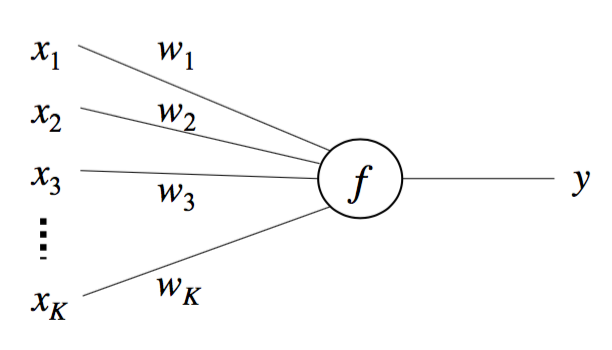
\includegraphics[width=0.65\textwidth]{../img/neuron.png}
  \caption[Mathematische Modellierung eines Neurons]{Mathematische Modellierung eines Neurons, auch bekannt als
  \emph{Perceptron}-Algorithmus. $x$ bezeichnet In-, $y$ den Output des Neurons, $w$ bilden die Gewichte und $f$ die
  Aktivierungsfunktion. Abbildung aus (\cite{rong2014word2vec}).\label{fig:perceptron}}
\end{figure}

Der Analogie der menschlichen Nervenzelle folgend erhält das Neuron mehrere Inputs in Form eines Vektors $x$ mit $K$
Dimensionen. Der Output erhält die Bezeichnung $y$. Um den Output zu bestimmen enthält die Zelle eine Aktivierungsfunktion
$f$ (um zu bestimmen, wann das Neuron ``feuert''):
\begin{equation}
  y = f(u)
\end{equation}

$u$ bezeichnet dabei einen Skalar, dem man durch das Summieren der mit $w$ gewichteten Inputs erhält:
\begin{equation}
  u = \sum_{i=0}^{K} w_i x_i = w^T x
\end{equation}

Für die Aktivierungsfunktion $f$ bieten sich mehrere Optionen. Ursprünglich wurde die \emph{Heaviside step function}
oder \emph{Rectifier (ReLU)} gewählt:
\begin{equation}
    f(u) = \begin{cases} 1 & \quad \text{if}\ u > 0 \\ 0 & \quad \text{otherwise} \\ \end{cases} \text{bzw.} \\
\end{equation}
\begin{equation}
  f(u) = max(0,u) = \begin{cases} 0 & \quad \text{if}\ u < 0 \\ u & \quad \text{otherwise} \end{cases}
\end{equation}

Andere Funktionen sind z.B. \emph{sigmoid} ($\sigma(u) \in [0,1]$)
und \emph{tanh} ($tanh(u) \in [-1, 1]$), im Gegenteil zu den beiden zuvor sind diese durch ihre s-förmige Form
kontinuierlich und dadurchableitbar:

\begin{equation}
  \sigma(u) = \frac{1}{1 + e^{-u}}
\end{equation}
\begin{equation}
  tanh(u) = \frac{e^{2u}-1}{e^{2u}+1}
\end{equation}

Um aus einzelnen Neuronen nun ein neurales Netzwerk zu kreieren, werden mehrere Schichten erstellt (i.d.R. eine Eingabe-
(\emph{input layer}), eine Ausgabe- (\emph{output layer}) und min. eine ``versteckte'' Schicht (\emph{hidden layer}).
Die Schichten bestehen dann aus mehreren Nervenzellen, wobei jede Zelle mit jeder anderen Zelle der vorhergehenden und
folgenden Schicht vernetzt ist (siehe Abbildung \ref{fig:neuralnet}).

\begin{figure}[h]
  \centering
  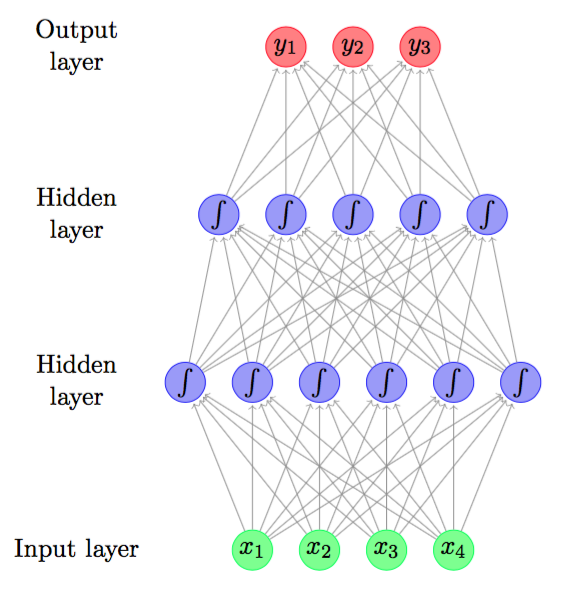
\includegraphics[width=0.5\textwidth]{../img/neuralnet.png}
  \caption[Darstellung eine neuralen Netzwerks]{Darstellung eines neuralen Netzwerks mit vier Schichten, davon jeweils eine
  für In- und Output, sowie zwei ``versteckte'' Schichten (\emph{hidden layer}). Bild aus (\cite{Goldberg15c}).\label{fig:neuralnet}}
\end{figure}

Die einzelnen Gewichtsvektoren $w$ aller Neuronen einer Schicht werden dann zu einer Gewichtsmatrix $W$ zusammengefasst,
wobei jede Zeile einem Gewichtsvektor entspricht. Zum Training dieser Strukturen wird der sog. \emph{Backpropagation}-
Algorithmus verwendet, der mithilfe einer vorher definierten Verlustfunktion (die anzeigt, inwiefern das durch das Netzwerk
erzeugt Ergebnis von dem erwünschtne Ergebnis abweicht) einen Fehler errechnet und diesen dann rekursiv durch alle
Schichten des Netzwerks zurückgibt und simultan die Werte innerhalb der Gewichtsmatrizen anpasst.

\section{Wortvektoren}

Frühere Experimente mit Wortvektoren arbeiteten meist mit sog. ``One-Hot''-Vektoren, bei denen jede Dimension i.d.R.
einem betimmten Wort zugeordnet wurde. Nehmen wir beispielsweise das Minikorpus \emph{Der Hund beißt den Mann} an.
Das Vokabular besteht dann aus $\textsc{V} = \{bei{\ss}t,\ Der,\ den,\ Hund,\ Mann\}$ (in alphabetischer Reihenfolge).
Um jedes dieser Wörter als einen der oben genannten Vektoren zu repräsentieren, können wir Vektoren der Länge $V$
($V$ steht eigentlich für $\|\textsc{V}\|$, wird der Übersicht halber aber im Folgenden stellvertrentend dafür verwendet)
benutzen. Um nun zum Beispiel einen Vektor für \emph{Hund} zu generieren, setzen wir den Wert der Stelle des Vektors (=
\emph{Feature}) auf $1$, der dem Index von Hund in $\textsc{V}$ entspricht,
also $\vec{v}(Hund)=(0, 0, 0, 1, 0)$.\\
Diese Art von Wortvektor wird gemeinhin als ``sparse'', also spärlich bezeichnet, da sie relativ wenig Information enthält.
Wortvektoren, die mithilfe von Neuralen Netzwerken trainiert werden (im Englischen zur Abgrenzung \emph{word embeddings}
genannt), beinhalten mehr (semantische) Informationen über das dazugehörige Wort, zudem lassen sich einzelne Features
nicht mehr auf eindeutig auf bestimmte Worte zurückführen.\\

Das Training dieser neuen Wortvektoren läuft folgendermaßen ab:
Als Input fungieren die erwähnten ``One-Hot''-Vektoren, welche genau so viele Dimensionen wie Worte im Vokabular besitzen
($\vec{v} \in \mathbb{R}^V$).
Die Modelle bestehen aus drei Schichten, namentlich \emph{Input}, \emph{Hidden} und \emph{Output}.
Input und Output besitzen die Dimensionalität von $V$), Hidden die von $N$.\\

\begin{figure}[h]
  \centering
  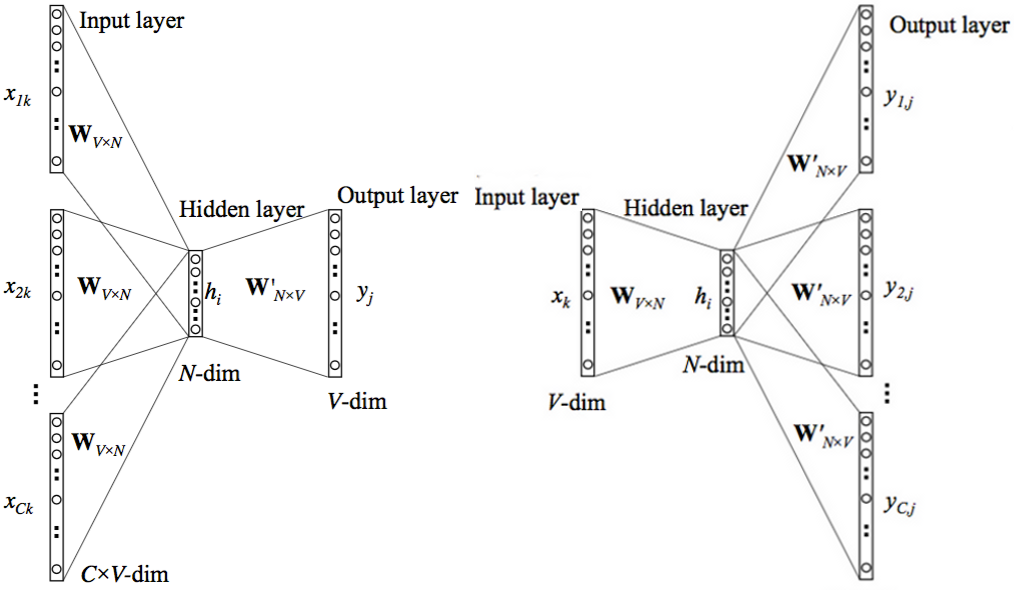
\includegraphics[width=1.1\textwidth]{../img/cbowskip.png}
  \caption[Gegenüberstellung von Skip-Gram und CBOW]{Gegenüberstellung der beiden Trainingsmethoden CBOW (links)
  und Skip-Gram (rechts). CBOW versucht die Wahrscheinlichkeit eines Wortes gegeben seines Kontexts zu trainieren,
  Skip-Gram die Wahrscheinlichkeit eines Kontextes gegeben eines Wortes.\label{fig:cbowskip}}
\end{figure}

Zwischen Input und Hidden liegt die Gewichtsmatrix $W$ und zwischen Hidden und Output die Matrix $W'$.
CBOW versucht, die Wahrscheinlichkeit eines Wortes gegeben eines Kontextes
der Größe $C$ zu maximieren (Kontext bezieht sich in diesem Fall auf die Summe der rechts und links vom Eingabewort stehenden
Wörter, siehe Abbildung \ref{fig:cbowskip}). Unsere Verlustfunktion, deren Wert es dabei zu minimieren gilt, besteht darin in der negativen logarithmischen
Wahrscheinlichkeit eines Wortes gegeben seines Kontextes:

\begin{equation}
  E = - log\ p(w_O | w_{I,1}, \ldots, w_{I,C})
\end{equation}

Beim Skip-gram-Modell verhält sich das Ganze genau umgekehrt, es wird versucht, den Kontext gegeben eines Eingabewortes
vorherzusagen:

\begin{equation}
  E = - log\ p(w_{I,1}, \ldots, w_O)
\end{equation}

In beiden Fällen wird daraufhin überprüft, ob die Vorhersage mit den tatsächlichen Daten übereinstimmt und die Abweichung
errechnet, mit der dann die Parameter der Gewichtsmatrizen $W$ und $W'$ rekursiv angepasst werden, um zukünftige Prognosen
zu verbessen, wofür der \emph{Backpropagation}-Algorithmus verwendet wird. Die Wortvektoren, die dann nach dem Abarbeiten aller Trainingsdaten resultieren, sind dann die Zeilen von
$W'$, wobei die \emph{i}-te Zeile der Matrix dem Wortvektor des Wortes mit dem Index \emph{i} im Vokabular entspricht.\\
Eigentlich erfordert das Training eine aufwendige Berechnung über alle Wörter des Vokabels, was der Skalierbarkeit dieses
Verfahrens entgegensteht. Der Aufwand kann allerdings durch Techniken wie \emph{Hierarchisches Softmax}, bei dem
der Aufwand durch einen binären Baum von $O(V)$ auf $O(log\ V)$ reduziert wird sowie
\emph{Negativem Sampling}. Bei letzterem werden ``schlechte'' (also Negativ-)Beispiele zum Training hinzugezogen,
woher sich auch der Name des Verfahrens ableitet.\\

%\section{Wortvektoren aus Dependenzen}
%
%Dependenzgrammatiken untersuchen die Abhängigkeiten zwischen Wörtern eines Satzes und fügen diese in eine Dependenzstruktur ein.
%Anders als in der Phrasenstrukturgrammatik entsteht dabei kein Syntaxbaum mit Knoten. Worte stehen in Abhängigkeitsverhältnissen,
%wobei das das die Dependenz verursachende Wort alt \emph{Regens}, das davon abhängige als \emph{Dependenz} bezeichnet wird.\\
%(\citeauthor{levy2014dependency}) machen sich dies zunutze, um den Kontext beim Training von Wortvektoren neu zu definieren:
%Er besteht nun nicht mehr als den umgebenden Wörtern im Satz, sondern aus den Depenzen: Für ein Word $w$ mit den Modifizierern
%$m_1, \ldots m_k$ und den Kopf $h$ besteht der Kontext nun aus $(m_1, lbl_1), \ldots (m_k, lbl_k), (h, lbl_h^{-1})$, wobei
%$lbl$ stellvertretend für eine Dependenzrelation steht, ein $-1$ im Exponenten zeigt das Inverse einer solchen Relation an.
%Ein Beispiel dafür ist in Abb. X zu sehen.\\

%\begin{figure}[h]
%    \centering
%    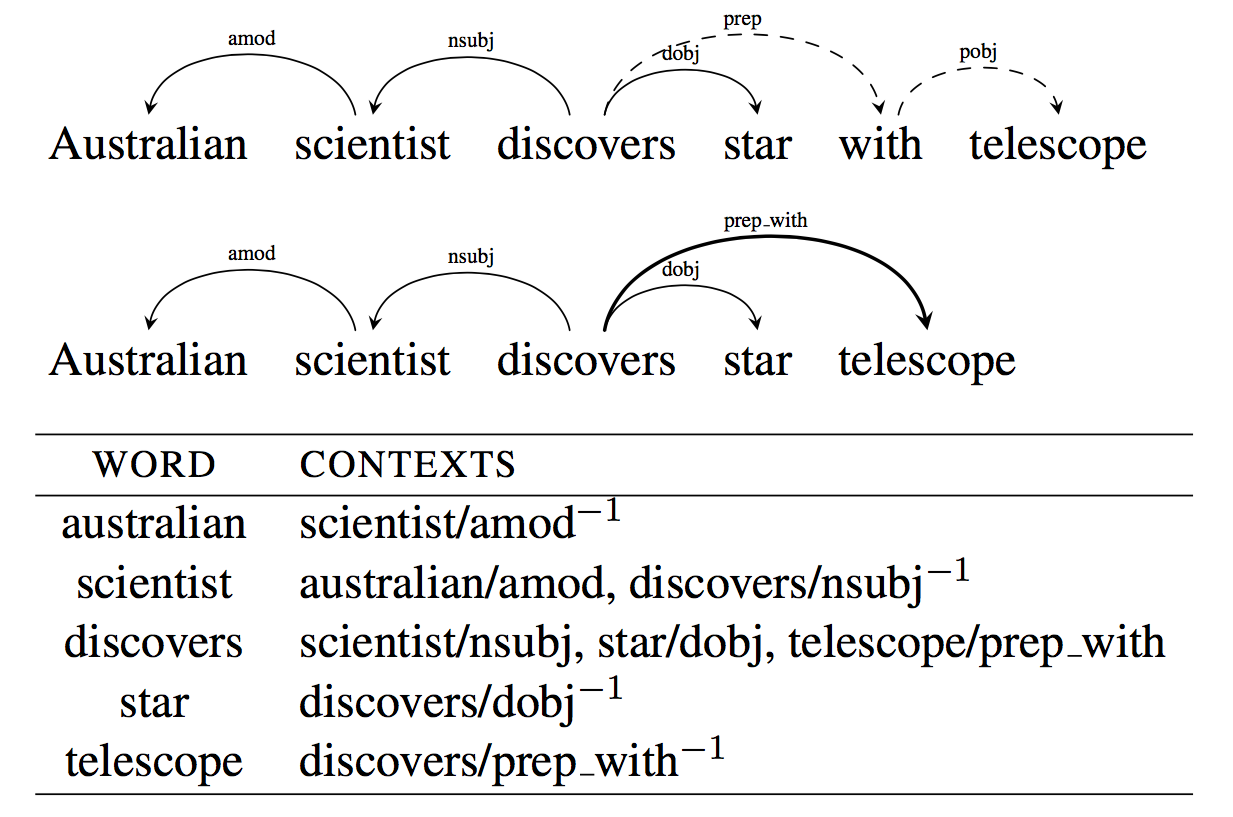
\includegraphics[scale=0.2]{../img/depend_ex.png}
%    \caption[Erstellung von Dependenzkontexten beim Wortvektortraining]{Beispiel der Erstellung von Wortkontexten aus Dependenzen.
%    Dependenzen mit Präposition werden zu einer Abhängigkeit zusammengefasst. \textbf{Oben}: Dependenzstruktur.
%    \textbf{Unten}: Extrahierte Kontexte.}
%\end{figure}

\section{Clustering}

\emph{Clustering} bezeichnet eine Art von unüberwachten maschinellen Lernen,
die versucht, Elemente, die nach vorher definierten Maßgaben als ähnlich erachtet
werden sollen, zu gruppieren.\\
Die Literatur zu diesem Thema bietet dabei eine Fülle von Algorithmen mit verschiedenen
Grundannahmen, aus denen es zu wählen gilt. Für die Aufgaben in dieser Arbeit wurde
der DBSCAN-Algorithmus (\textbf{D}ensity-\textbf{B}ased \textbf{S}patial \textbf{C}lustering of
\textbf{A}pplications with \textbf{N}oise) gewählt, da er folgende Kriterien erfüllt:
\begin{itemize}
  \item DBSCAN erlaubt es, dass nicht alle Datenpunkte bei der
  Terminierung des Algorithmus einem Cluster zugeordnet sein müssen (\emph{Outlier detection})
  \item Die Anzahl der Cluster muss bei Beginn des Algorithmus nicht festgelegt werden.
  \item Cluster werden nicht nach der räumlichen Distanz zwischen den Punkten gebildet, sondern nach deren
  Dichte im Raum. Dies lässt auch nicht-sphärische Clusterformen zu.
\end{itemize}

Zur Erklärung von DBSCAN müssen zuerst einige Definitionen erstellt werden (siehe Abbildung \ref{fig:dbscan} zur visuellen
Darstellung):
\begin{itemize}
  \item Ein Punkt $p$ in den Daten wird dann als
  Kernpunkt (\emph{core point}) bezeichnet, sofern mindesten $minPts$ Punkte innerhalb einem Radius $\epsilon$ vorhanden sind.\\
  Diese Punkte sind von $p$ \emph{direkt erreichbar}.
  \item Ein Punkt $q$ ist von $p$ erreichbar, sofern es einen Pfad $p_1, \ldots, p_n$ mit $p_1 = p$ und $p_n = q$ gibt, wobei
  jeder Punkt $p_{i+1}$ von einem Punkt $p_i$ direkt erreichbar ist.
  \item Alle Punkte, die nicht von einem anderen Punkt aus direkt erreichbar sind, sind Ausreißer (\emph{Outlier}).
  \item Zwei Punkte $p$ und $q$ sind \emph{direkt verbunden}, sofern es einen Punkt $o$ gibt,
  von dem aus beide Punkte direkt erreichbar sind.
  \item Cluster bestehen aus Punkten, die alle miteinander direkt verbunden sind.
\end{itemize}

\begin{figure}[h]
  \centering
  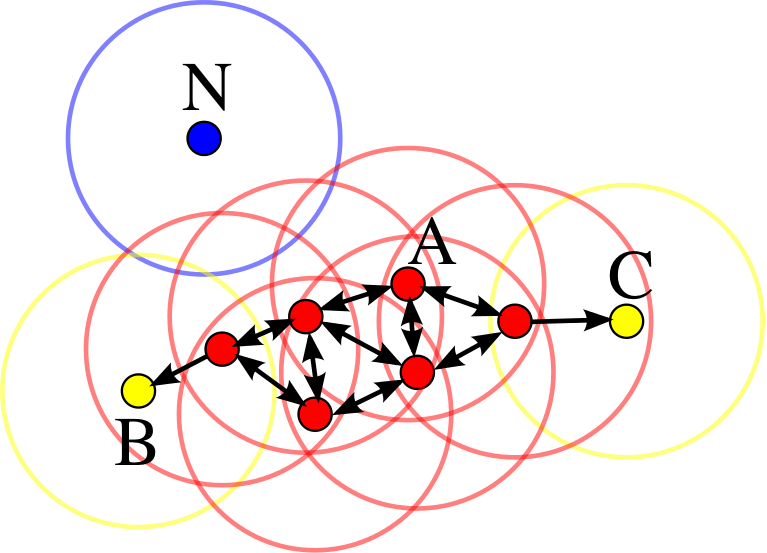
\includegraphics[width=0.6\textwidth]{../img/DBSCAN-Illustration.png}
  \caption[Darstellung der Funktionsweise von DBSCAN]{Darstellung der Funktionsweise von DBSCAN. Punkt A ist ein Kernpunkt, die
  Punkte B und C sind von A aus erreichbar. Punkt N ist nicht erreichbar und damit ein Ausreißer.\label{fig:dbscan}\footnotemark}
\end{figure}
\footnotetext{Abbildung von
Chire - Eigenes Werk, CC BY-SA 3.0, \url{https://commons.wikimedia.org/w/index.php?curid=17045963} (zuletzt abgerufen am
25.04.16).}

Der Algorithmus ist von linearer Komplexität, sofern ihm eine geeignete Indexierung der Daten zugrunde gelegt wird, ansonsten
verhält sich die Komplexität quadratische zur Anzahl der Datenpunkte\footnote{Bei der
\verb|scikit-learn|-Implementation wird beispielsweise ein Nearest-Neighbour-Graph verwendet:
\url{http://scikit-learn.org/stable/modules/generated/sklearn.cluster.dbscan.html} (zuletzt abgerufen am 25.04.16)}.

% Chapter 4

\chapter{Vorbereitung} % Main chapter title

\label{Chapter4} % For referencing the chapter elsewhere, use \ref{Chapter1}

%----------------------------------------------------------------------------------------

\section{Vorbereitung}

  Für die nachfolgenden Experimente in den Kapiteln \ref{Chapter6}, \ref{Chapter7} und \ref{Chapter8}
  mussten einige Daten zuerst beschafft und unter Umständen aufbereitet werden. Die ergriffenen Maßnahmen werden
  deshalb in diesem Kapitel beschrieben.

  \subsection{Verwendete Daten}

  Die anfangs verwendeten Daten lassen sich grob in vier Kategorien einteilen: Den Korpus, das Relationsdatenset,
  Wortähnlichkeitslisten sowie Analogiedatensets (siehe Abbildung \ref{fig:datasets}).\\
  Als Korpus wurde der \textsc{DECOW14X}-Korpus verwendet. Genaueres über dessen Beschaffenheit und Vorverarbeitung für das
  Training von Wortvektoren werden in \ref{sec:corpusprep} und \ref{sec:vectrain} beschrieben.

  \begin{figure}[h]
    \centering
    \def\arraystretch{1.5}
    \resizebox{\textwidth}{!}{%
    \begin{tabular}{l|l|rl|l}
      \textsc{Art} & \textsc{Name} & \multicolumn{2}{l|}{\textsc{Beschreibung}} & \textsc{Quelle} \\
      \hline \hline
      Korpora & \textsc{DECOW14X} & \multicolumn{2}{l|}{Deutschsprachiger Webkorpus} & (\cite{schafer2012building}) \\
      \hline
      Relationsdaten & \textsc{FB14k} & \multicolumn{2}{l|}{592k Relationstripel aus Freebase} & (\cite{bordes2013translating}) \\
      \hline
      \multirow{4}{*}{\parbox[t]{1.5cm}{Wortähnlich-keiten}} & \textsc{Schm280} & 280 & \multirow{4}{*}{\Vast \} \parbox[c]{4cm}{nach Ähnlichkeit bewertete Wortpaare}} & (\cite{koper2015multilingual})\\ \cline{5-5}
       & \textsc{Wortpaare65} & 65 & & \multirow{3}{*}{(\cite{rubenstein1965contextual})} \\
       & \textsc{Wortpaare222} & 222 & & \\
       & \textsc{Wortpaare350} & 350 & & \\
      \hline
      \multirow{2}{*}{Analogien} & \textsc{Google} & \multicolumn{2}{l|}{Datenset mit 18.552 Analogien} & \multirow{2}{*}{(\cite{koper2015multilingual})} \\
       & \textsc{SemRel} & \multicolumn{2}{l|}{Datenset mit 2.462 Analogien} & \\
    \end{tabular}%
    }
  \caption[Übersicht über verwendete vorgefertigte Datensets]{Übersicht über in dieser Arbeit verwendete, extern generierte
  Datensets sowie deren Quelle.\label{fig:datasets}}
  \end{figure}

  Relationsdaten aus der mittlerweile in \text{Wikidata} integrierten Wissensdatenbank\footnote{Siehe
  \url{https://plus.google.com/109936836907132434202/posts/bu3z2wVqcQc} (zuletzt abgerufen am 21.07.16).}
   \textsc{Freebase} wurden im Datenset \textsc{FB14k} von (\cite{bordes2013translating}) gesammelt.
  Diese werden vor allem in den Versuchen von Kapiteln \ref{Chapter6} und \ref{Chapter8} relevant.\\
  Alle anderen Datensets sind zur Evaluation der Wortvektoren in Kapitel \ref{sec:we-eval} angedacht: Die Sets
  \textsc{Schm280}, \textsc{Wortpaare65}, \textsc{Wortpaare222} und \textsc{Wortpaare350} bestehen aus einer Reihe
  von Wortpaaren, die von menschlichen Annotatoren auf verschiedenen Skalen nach Ähnlichkeit bewertet wurden.\\
  \textsc{Google}\footnote{Eigentlich: \textsc{Google semantic/syntactic analogy datasets}} und \textsc{SemRel} sind
  in verschiedene Kategorien eingeteilte Analogiepaare der Form ``W verhält sich zu X wie Y zu Z''. Bei der Evaluation
  wird dann die Fähigkeit eines Systems mit Wortvektoren getestet, diese korrekt zu vorvervollständigen, wenn Z nicht
  gegeben ist.


  \subsection{Aufbereitung des Korpus}\label{sec:corpusprep}

  Als Textressource wurde das DECOW14X-Korpus (DE = Deutsch, COW = ``\textbf{CO}rpus from the \textbf{W}eb'') verwendet.
  Dieses Korpus von (\cite{schafer2012building}) besteht aus 21 Teilkorpora,
  die in den Jahren 2011 und 2014 von deutschsprachigen Internetseiten extrahiert und aufbereitet wurden. Diese beinhalten
  Informationen im Bezug auf PoS-Tagging, Chunking, Lemmatisierung, Eigennamen (\emph{named entities}) und einige Metadaten.
  Die Sätze liegen im \textsc{CoNLL}-Format\footnote{Siehe \url{http://ilk.uvt.nl/conll/} (zuletzt abgerufen am 11.04.16)} vor,
  wobei jedem Wort und dessen Annotationen eine ganze Zeile gewidmet ist.
  Stazgrenzen werden durch XML-Tags getrennt. Summa summarum enthält das Korpus 624.767.747 Sätze mit 11.660.894.000 Tokens.\\

  Für diese Arbeit wurden auf Basis der Ressource zwei Versionen für das Training der Wortvektoren erstellt:
  \begin{itemize}
      \item Eine Datei mit den originalen Tokens durch Leerzeichen getrennt, je ein Satz pro Zeile.
      \item Eine Datei mit den lemmatisierten Tokens durch Leerzeichen getrennt, je ein Satz pro Zeile.
  \end{itemize}

  Um die beiden Varianten zu erstellen, wurden die jeweils relevanten Informationen aus den dazugehörigen Spalten des
  \textsc{CoNLL}-Formats verwendet.\\
  Darüber hinaus wurden für spätere Anwendungen in Kapitel \ref{Chapter7} alle Eigennamen sowie die Satz-IDs für
  alle Eigennamen gesammelt (siehe die Kookkurrenzeinschränkung \ref{form:lambda-cooc}).

  \subsection{Training der Wortvektoren}\label{sec:vectrain}

  Wortvektoren werden mithilfe des Tools \verb|word2vec| und zwei verschiedenen Modellen trainiert: Continuous-Bag-of-Words (CBOW)
  und Skip-Gram. Das CBOW-Model wurde zuerst von (\cite{mikolov2013efficient}) vorgestellt. Die Erklärung der Funktionsweise
  wird im nachfolgenden Teil recht klein gehalten, für eine ausführlichere und verständliche Ausführung wird beispielsweise
  die Arbeit von (\cite{rong2014word2vec}) oder die Ausführung in Kapitel \ref{sec:wordvec} empfohlen.\\

  Als Eingabe benötigt es eine Textressource, die einen Satz pro Zeile enthält, Tokens durch Leerzeichen getrennt und gibt die Wortvektoren
  entweder einem einfach Text- oder Binärformat aus.\\
  Das Tool lässt zudem dem Nutzer offen, einige Parameter zu verändern. Jene, die in dieser Arbeit berücksichtigt wurden, sollen
  dabei näher erläutert werden:
  \begin{itemize}
    \item \verb|-sample|\\Die Wahrscheinlichkeit, mit der Einfluss hochfrequenter Worte im Training geregelt wird
    \item \verb|-cbow|\\Bestimmt, welche Trainingsmethode verwendet wird ($0\ \hat{=}$ Skip-gram, $1\ \hat{=}$ Continuous-Bag-of-Words)
    \item \verb|-negative|\\Anzahl von negativen Beispielen beim Training.
  \end{itemize}

  Zwar bietet das Tool auch noch andere Parameter, jedoch soll aufgrund der Empfehlungen in (\citeauthor{levy2015improving}), in
  der eine große Anzahl von Konfigurationen ausprobiert wurde, im Rahmen dieser Arbeit nur mit den oben genannten Werten experimentiert werden.
  Weiterführende Optimierungen wurden zudem unterlassen, um den Rahmen dieser Arbeit nicht zu sprengen.


\section{Evaluationsarten für Wortkontextvektoren}\label{sec:we-eval}

An dieser Stelle sollen die verschiedenen Ansätze zum Evaluieren von Wortkontextvektoren miteinander verglichen werden. Zu diesem Zweck sollte zuerst eine Frage gestellt werden:
Was macht eine Menge von Wortkontextvektoren ``besser'' bzw. ``schlechter'' als andere?\\
Da der Vorteil von Wortkontextvektoren darin besteht, semantische Information zu beinhalten, wird diese
Frage meist dahingehend beantwortet, dass Vektoren dann als überlegen anzusehen sind, wenn sie
eine höhere semantische ``Ausdruckskraft'' besitzen. Um diese festzustellen, haben sich in Veröffentlichungen
zu diesem Thema bestimmte Vorgehensweisen durchgesetzt, die in den folgenden Abschnitten, vorgestellt, erläutert,
angewendet und kritisch reflektiert werden sollen.\\

  \subsection{Qualitative Evaluation}

  Qualitative Verfahren zur Evaluation sind meist recht simple Ansätze, die für das menschliche
  Auge leicht zu interpetierende Ergebnisse liefern. Deshalb sind sie für einen ersten Eindruck
  auch durchaus geeignet, sollten wenn möglich aber nicht als alleinige Kriterium für eine Bewertung
  verwendet werden, da sie meistens nur einen kleinen Ausschnitt aller in den Ergebnissen enthaltenen
  Informationen darstellen können. \\
  Beim Beispiel der Wortkontextvektoren werden beispielsweise einige Wörter des Vokabulars stellvertretend ausgewählt
  und zu diesen die \emph{k} nächsten Nachbarn\footnote{I.d.R. basierend auf der euklidischen Distanz.} im Vektorraum gesucht.
  Unter der Annahme, dass in Vektorräumen von Wortkontextvektoren ähnliche Wörter nahe beieinanderliegen, sollte diese Liste
  im Idealfall eng verwandte Begriffe zutage fördern (siehe Abbildung \ref{fig:wortliste}).\\

  \begin{figure}[h]
    \centering
    \begin{changemargin}{0cm}{0cm}
    \resizebox{\textwidth}{!}{%
    \begin{tabular}{c|cccc}
      \textsc{Nr.} & \textsc{Frankreich} & \textsc{Bank} & \textsc{Computerlinguistik} & \textsc{gekratzt} \\
      \hline \hline
      \multirow{5}{*}{\Romannum{1}} & \textsc{Belgien} & \textsc{Anlagebank} & \textsc{Linguistik} & \textsc{gekrazt} \\
       & \textsc{Italien} & \textsc{(unknown)\_Bank} & \textsc{Informationswissenschaft} & \textsc{weggekrazt} \\
       & \textsc{Niederland} & \textsc{BAnk} & \textsc{Texttechnologie} & \textsc{geschubbert} \\
       & \textsc{Niederlande} & \textsc{Bankstatus} & \textsc{Sprachwissenschaft} & \textsc{gekratz} \\
       & \textsc{Spanien} & \textsc{Geldinstitut} & \textsc{Softwaretechnik} & \textsc{abgeleckt} \\
      \hline
      \multirow{5}{*}{\Romannum{8}} & \textsc{Italien} & \textsc{Hausbank} & \textsc{Bioinformatik} & \textsc{gekrazt} \\
      & \textsc{Ungarn} & \textsc{Geschäftsbank} & \textsc{Texttechnologie} & \textsc{weggekrazt} \\
      & \textsc{Polen} & \textsc{Großbank} & \textsc{Informationswissenschaft} & \textsc{geschubbert} \\
      & \textsc{Spanien} & \textsc{Kreditbank} & \textsc{Softwaretechnik} & \textsc{angeknabbert} \\
      & \textsc{Belgien} & \textsc{Mutterbank} & \textsc{Linguistik} & \textsc{rausgerissen} \\
      \hline
      \multirow{5}{*}{\Romannum{22}} & \textsc{Italien} & \textsc{Kreditinstitut} & \textsc{Bioinformatik} & \textsc{geritzt} \\
      & \textsc{Ungarn} & \textsc{Geldinstitut} & \textsc{Wirtschaftsgeographie} & \textsc{angesengt} \\
      & \textsc{Polen} & \textsc{Sparkasse} & \textsc{Grundschulpädagogik} & \textsc{zusammengenäht} \\
      & \textsc{Spanien} & \textsc{Landesbank} & \textsc{Computerwissenschaft} & \textsc{aufgesprungen} \\
      & \textsc{Belgien} & \textsc{Finanzinstitut} & \textsc{Humangeographie} & \textsc{tupfen} \\
    \end{tabular}%
    }
  \end{changemargin}
    \caption[Listen der \emph{k} nächsten Nachbarn von Wörtern in verschiedenen Datensets]{Listen der \emph{k} nächsten Nachbarn von Wörtern in verschiedenen Datensets. Inspiriert
            von (\cite{collobert2011natural}). \label{fig:wortliste}}
  \end{figure}

  Das Problem bei dieser Methode liegt in der menschlichen Subjektivität: Die präsentierte Auswahl der Begriffe
  muss nicht zwangsläufig repräsentativ für die restlichen Daten sein und könnte theoretisch aus den wenigen,
  gut funktionierenden Beispielen bestehen. Darüber hinaus bleibt es in einigen Fällen schwierig,
  die Ergebisse verschiedener Datensets zu vergleichen, da sich die Qualität der \emph{k} Nachbarn
  nicht quantifizieren lässt: Es lässt sich vielleicht erkennen, das diese in einem Fall wenig Sinn machen und
  im anderen Fall die Erwartungen erfüllen; an anderer Stelle scheinen die Resultate für den Betrachter jedoch nicht
  unbedingt schlechter, sondern einfach nur anders.\\
  Darum ist wiederum festzuhalten, dass sich qualitative Methoden in diesem Fall eher für den ersten Eindruck
  eignen, weiterhin aber Prozeduren mit quantifizierbaren Ergebnissen verwendet werden sollten, wie z.B.
  nächsten Abschnitt \ref{sec:quanteval} beschrieben werden.

  \subsection{Quantitative Evaluation}\label{sec:quanteval}

  Bei der quantitativen Evaluation von Wortkontextvektoren werden die folgenden Ideen aufgegriffen:\\
  \begin{enumerate}
    \item \textbf{Benchmark-Tests}\\
      Bei dieser pragmatischen Art der Bewertung werden wird das Datenset als Grundlage für
      einfach Aufgaben wie Sentiment-Klassifikation oder Part-of-Speech-Tagging verwendet.
      Die Qualität der Daten wird dann anhand der Ergebnisse des Systems gemessen.\\
      Diese extrinische Evaluationsmethode macht ergo nur dann Sinn, wenn man mehr als ein Datenset
      miteinander vergleicht. Dabei muss sichergestellt werden, dass die Tests immer unter den
      selben Bedingungen ablaufen, damit eine Vergleichbarkeit gewährleistet bleibt.\\
    \item \textbf{Wortähnlichkeit}\\
      Hierbei werden Wortpaaren Ähnlichkeitswerte von menschlichen Annotatoren zugeordnet. Anschließend
      werden mit den zu Verfügung stehenden Vektoren Ähnlichkeitswerte für die gleichen Paare berechnet,
      in der Regel mithilfe der Kosinus-Ähnlichkeit. Diese beschreibt die Ähnlichkeit zweier Vektoren
      als den Winkel zwischen ihnen, mit einem Wert von $-1$ ($\hat{=} 180^{\circ}$ bzw. komplett unterschiedlich) über 0
      ($\hat{=} 90^\circ$) und $+1$ ($\hat{=} 0^\circ$ bzw. Äquivalenz):
      \begin{equation}\label{form:cossim}
        cos(\vec{a}, \vec{b}) = \frac{\vec{a} \cdot \vec{b}}{\|\vec{a}\| \|\vec{b}\|}
      \end{equation}
      Danach kann mit \emph{Spearman's $\rho$}
      \footnote{Auch \emph{Spearman's rank correlation coefficient}.
      Berechnet wird dieser für zwei Mengen von Datenpunkten $X=\{x_i\}^n_{i=1}$ und $Y=\{y_i\}^n_{i=1}$ durch
      \[
      r_s = \frac{\sum_i(rg(x_i)-\overline{rg}_x)(rg(y_i)-\overline{rg}_y)}{\sqrt{\sum_i(rg(x_i)-\overline{rg}_x)^2} \sqrt{\sum_i(rg(y_i)-\overline{rg}_y)^2}}
      \]
      wobei jedem Wert $x_i$ und $x_j$ ein Rang $rg(\cdot)$ zugewiesen wird. $\overline{rg}_{(\cdot)}$ entspricht dem durchschnittlichen
      Rang.
      }.
      anschließend festgestellt werden, ob die beiden Werte für die Wortpaare korrelieren, sprich ob
      das System Paaren, denen von Menschen ein hoher Ähnlichkeitswert zugewiesen wurde, auch eine hohe
      Ähnlichkeit zuschreibt. Dabei zeigt $\rho \in [-1, 1]$ den Grad der Korrelation, wobei
      $-1$ einer starken negativen, $+1$ einer starken positiven Korrelation entspricht.
    \item \textbf{Analogien}\\
      Die dritte Methode basiert auf Analogien der Form \emph{a verhält sich zu a' wie b zu b'}.
      Die Daten werden nun dahingehend getestet, indem unter Gebrauch der Cosinus-Ähnlichkeit
      das $\tilde{b}$ aus dem Vokabular $\mathcal{V}$ gesucht wird, welches besonders ähnlich zu $b$ und $a'$ aber unähnlich zu $a$ ist:
      \begin{equation}
        b' = \underset{\tilde{b}\ \in\ \mathcal{V}}{argmax}\ cos(\tilde{b}, b - a + a')
      \end{equation}
      Sind alle Vektoren der Länge eins, so kann diese Gleichung aufgrund der obigen Definition der Kosinusähnlichkeit
      (\ref{form:cossim}) umformuliert werden:
      \begin{equation}
        b' = \underset{\tilde{b}\ \in\ \mathcal{V}}{argmax}\ cos(\tilde{b}, b) - cos(\tilde{b}, a) + cos(\tilde{b}, a')
      \end{equation}
      Diese Methode wird gemeinhin als \textsc{3CosAdd} bezeichnet. (\cite{levy2014linguistic}) etablierten dazu jedoch
      eine Alternative namens \textsc{3CosMul}\footnote{Um nur Werte im Bereich $[0,1]$ zu erhalten, wird die Formel
      für die Kosinusähnlichkeit folgendermaßen angepasst:
      \[
        cos'(\vec{a}, \vec{b}) = \frac{cos(\vec{a}, \vec{b}) + 1}{2}
      \]}, die bei Tests bessere Ergebnisse produziert:
      \begin{equation}
        b' = \underset{\tilde{b} \in \mathcal{V}}{argmax} \frac{cos'(\tilde{b}, b)\ cos'(\tilde{b}, a')}{cos'(\tilde{b}, a) + \epsilon}
      \end{equation}
      Dabei ist $\epsilon = 0,001$, um die Divison durch Null zu verhindern.\\
      Der Erfolg der Evaluation kann dann als Anteil der richtig vervollständigten Analogien (bei denen $\tilde{b}^* = b^*$) gemessen werden.
  \end{enumerate}
  In dieser Arbeit sollen die Datensets durch die zweit- und drittgenannte Methode evaluiert werden.
  Ein weiterer Fallstrick liegt allerdings in der Zusammenstellung der Datensets: So liefern
  die genannten Evaluationsdatensets nur dann aussagekräftige Ergebnisse, wenn bei der Wortähnlichkeit die menschlichenen
  Annotatoren zuverlässig und sinnvoll die Paare bewertet haben (zu messen z.B. mit $Cohen's\ \kappa$) und bei
  den Analogien aus der Zusammenstellung ebendieser (soll heißen: Welche Entitäten sind enthalten? Wie oft kommen diese
  im Datenset vor? Welche semantische Relationen wurden ausgewählt? Wurden diese maschinell oder per Hand erzeugt?).\\
  Aus diesem Grund sollen die benutzten Evaluationssets im hierauf folgenden Abschnitt \ref{sec:evaldata} näher beleuchtet werden.

  \subsection{Evaluationsdaten}\label{sec:evaldata}

    \subsubsection{Wortpaarähnlichkeit}

    Im Englischen wird für die Wortähnlichkeitsevaluation häufig das \textsc{WordSim353}-Datenset von (\cite{finkelstein2001placing})
    verwendet. Dieses wurde unter dem Namen \textsc{Schm280} in deutsche portiert, wobei die Paare nicht nur einfach übersetzt, sondern die
    Ähnlichkeit auch noch von deutschen Muttersprachlern neu bewertet wurde. Es enthält insgesamt 280 Wortpaare.\footnote{Es konnte
    jedoch nicht festgestellt werden, wieviele Menschen die Wortpaare neu bewertet haben. Während des Übersetzungsschritts
    wurde eine Zahl von 12 Teilnehmern angegeben, ob jedoch genauso viele im Bewertungsschritt partizipiert haben und wie groß
    ihre Übereinstimmung war, ist nicht festzustellen.}\\ \\
    \textsc{Wortpaare65}, \textsc{Wortpaare222} und \textsc{Wortpaare350} entstammen der Arbeit von (\cite{rubenstein1965contextual}).
    Dabei werden Wortpaaren
    Werte von 0 ($\hat{=}$ vollkommen unzusammenhängend) bis 4 ($\hat{=}$ stark zusammenhängend) zugeschrieben. Die Anzahl
    der menschlichen Annotatoren sowie deren Übereinstimmung in Form von $Cohen's\ \kappa$\footnote{
    Dies ist definiert als
    \[
      \kappa = \frac{A_o - A_e}{1 - A_e}
    \]
    wobei $A_o$ die beobachtete Übereinstimmung der Annotatoren und $A_e$ die statistisch zu erwartende Übereinstimmung
    der Annotatoren bezeichnet.
    } sind in Abbildung \ref{fig:evalsets} festgehalten.

    \begin{figure}[h]
      \centering
      \begin{tabular}{l|cc}
        \textsc{Datenset} & \textsc{\#Annotatoren} & $\kappa$ \\
        \hline
        \textsc{Schm280} & 12 (?) & ??? \\
        \textsc{Wortpaare65} & 24 & 0,81 \\
        \textsc{Wortpaare222} & 21 & 0,49 \\
        \textsc{Wortpaare350} & 8 & 0,69 \\
      \end{tabular}
      \caption[Anzahl der Annotatoren und Agreement der Wortähnlichkeitsdatensets]{Anzahl der Annotatoren und Agreement (als $Cohen's\ \kappa$) der Wortähnlichkeitsdatensets.
      \label{fig:evalsets}}
    \end{figure}

    \subsubsection{Analogien}

    Die \textsc{Google semantic/syntactic analogy datasets} wurden von (\cite{mikolov2013efficient}) eingefügt und bestehen
    aus Analogien der Form \emph{a verhält sich zu a' wie b zu b'}. (\cite{koper2015multilingual}) haben diese manuell übersetzt und durch
    drei menschliche Prüfer validieren lassen. Dabei wurde die Kategorie ``adjektiv - adverb'' ausgelassen, da sie
    im Deutschen nicht (im gleichen Ausmaß wie im Englischen) existiert, wodurch 18.552 Analogien übrigbleiben. Diese werden im Folgenden einfach als
    \textsc{Google} bezeichnet.\\ \\
    \textsc{SemRel} wurde aus Synonomie-, Antonomie- und Hypernomie-Beziehungen von (\cite{koper2015multilingual}) für das Deutsche und Englische
    konstruiert. Dabei werden Substantive, Verben und Adjektive berücksichtigt. In der deutschen Variante sind 2.462
    (recht schwierige zu vervollständigende) Analogien enthalten, die aus teilweise sehr seltenen Wörter kreiert wurden
    (siehe eine Kritik dazu im nächsten Abschnitt\ref{sec:evalerg}).

  \subsection{Evaluationsergebnisse}\label{sec:evalerg}

  Im Folgenden sollen die Ergebnisse der Wortkontextvektor-Evaluation diskutiert werden. Am Ende dieses Abschnitts werden dabei
  nur die Datensets mit den besten Ergebnissen und deren Konfiguration von Parametern vorgestellt, eine ausführliche
  Übersicht findet sich aber im Appendix \ref{AppendixB}.\\

%Mark I     & \textbf{-0,8096}         & \textbf{-0,4640$_{(13)}$}   & \textbf{-0,7302$_{(13)}$}   & \textbf{-0,7094$_{(2)}$}  & \textbf{44,56}  & 1,71 \\
%Mark XIII  & \textbf{-0,8247$_{(1)}$} & \textbf{-0,5066$_{(102)}$}  & \textbf{-0,7494$_{(132)}$}  & -0,7097$_{(48)}$          & 15,51           & \textbf{3,01} \\
%Mark XIV   & -0,8106$_{(1)}$          & -0,4953$_{(102)}$           & -0,7362$_{(132)}$           & \textbf{-0,7205$_{(48)}$} & 14,51           & 2,56 \\

  \begin{figure}[h]
    \centering

    \resizebox{\textwidth}{!}{%
    \begin{tabular}{l||l|l|l|l||l|l}
      \textsc{Nr.} & \textsc{Wortpaare65} & \textsc{Wortpaare222} & \textsc{Wortpaare350} & \textsc{Schm280} & \textsc{Google} & \textsc{SemRel} \\
      \hline
      \Romannum{1} & \textbf{-0,8096} & \textbf{-0,4640$_{(13)}$} & \textbf{-0,7302$_{(13)}$} & \textbf{-0,7094$_{(2)}$} & \textbf{44,56}  & 1,71 \\
      \Romannum{13} & \textbf{-0,8247$_{(1)}$} & \textbf{-0,5066$_{(102)}$}  & \textbf{-0,7494$_{(132)}$} & -0,7097$_{(48)}$ & 15,51 & \textbf{3,01} \\
      \Romannum{14} & -0,8106$_{(1)}$ & -0,4953$_{(102)}$ & -0,7362$_{(132)}$ & \textbf{-0,7205$_{(48)}$} & 14,51 & 2,56 \\
    \end{tabular}%
    }

    \caption[Evaluationsergebnisse der besten Vektordatensets]{Evaluationsergebnisse der drei besten Vektordatensets. Links:
    Bewertung durch Spearman's $\rho$. Rechts: Treffer beim Vervollständigen
    von Analogien in Prozent. Nicht gefundene Wortkontextvektoren klein in Klammern hinter dem Wert. Für eine vollständige Liste
    der Trainingsparameter jedes Datensets siehe \ref{AppendixA}. Für die gesamte Liste aller Ergebnisse siehe \ref{AppendixB}.}
  \end{figure}

  Nach der Evaluation war zuallererst festzustellen, dass sowohl bei Datensets, die auf dem normalen oder lemmatisierten Korpus
  trainiert wurden, Ergebnisse mit steigender Downsamplingrate schlechter wurden. Dies war sowohl bei Training mit dem CBOW- als
  auch mit dem Skip-Gram-Modell feststellbar. Darüber hinaus lieferte Letzteres im Schnitt bessere Resultate (und benötigte
  während des Trainings auch weniger Zeit). Das Lemmatisieren führte dazu, das während der Bewertung der Sets oft einige
  Schritte nicht durchgeführt werden könnten, was anhand der in Subskript in Klammern stehenden Zahlen abzulesen ist.
  Darunter leidet leider auch wenig die Vergleichbarkeit; es erscheint aber zumindest logisch, dass bei gleichem Evaluationswert
  einem Datenset mit weniger nicht gefundenen Wortkontextvektoren eine höhere Qualität beizumessen ist. Je nach
  späterem Anwendungsgebiet kann diese Unterscheidung aber nicht relevant sein.\\
  Bei den Analogie-Datensets sind ähnliche Tendenzen sichtbar: Beim \textsc{Google}-Datenset sind die Diskrepanzen jedoch
  deutlich stärker und Vektoren des unlemmatisierten Korpus schneiden deutlich besser ab, was vor allem dadurch
  zu erklären ist, dass in diesem Set auch Flektion geprüft wird (bspw. \emph{schreiben} verhält sich zu \emph{schreibt} wie
   \emph{sagen} zu \emph{sagt}) und diese Formen durch die Lemmatisierung velorengehen. Beim \textsc{SemRel}-Datenset
  verhält sich das ganze allerdings genau umgekehrt, wenn auch die Unterschiede wesentlich feiner sind. Da hier für alle
  möglichen Formen eines Wortes nur eine Vektorrepräsentation trainiert wird, ist zu schließen, dass diese dann auch
  mehr Information in sich kodiert.\\

  Es ist ferner zu erkennen, dass einige der extern bereitgestellten Evaluationsdaten nicht sehr gut zusammengestellt wurden.
  Bei \textsc{Wortpaare222} prägen sich die Korrelationswerte nicht unter $-0,54$ aus, was dafür spricht, das die Ähnlichkeit
  der Wortpaare für sowohl für das System als möglicherweise auch für die menschlichen Annotatoren schwer einzuschätzen war
  \footnote{Beispielhaft seien hier einige Wortpaare aus \textsc{Wortpaare222} genannt, die nach Ähnlichkeit bewertet werden
  mussten, um das Problem zu illustrieren:\\
  \emph{wahrnehmen} - \emph{Grundsatzfrage} / \emph{groß} - \emph{Arbeitszeitregelung} /
  \emph{Hubschraubertyp} - \emph{einschließlich} / \emph{Büroequipment} - \emph{Institut}.}
  Beim \textsc{SemRel}-Analogienset sticht dieser Fakt noch viel drastischer heraus: Im besten Fall wurden $3\%$ (sic!)
  der Analogien richtig vom System vervollständigt. Es sei angemerkt, dass es auch dem Autor und anderen gefragten Personen
  schwerfiel, stichprobenartig ausgewählte Fragen richtig zu beantworten
  \footnote{\emph{Lieblichkeit} verhält sich zu \emph{Anmut} wie \emph{Mittelklasse} zu$\ldots$? \rotatebox[origin=c]{180}{\emph{Mittelschicht}}\\
  \emph{Zivilgesellschaft} verhält sich zu \emph{Bürgergesellschaft} wie \emph{Gegenargument} zu$\ldots$? \rotatebox[origin=c]{180}{\emph{Widerspruch}}\\
  \emph{Trio} verhält sich zu \emph{Solo}  wie \emph{Arzt} zu$\ldots$? \rotatebox[origin=c]{180}{\emph{Patient}}}.
  Deshalb stellen sich die Ergebnisse bei diesem Vergleichsset ohne klare Tendenz in den Resultaten und generell sehr schlecht dar.\\

  Für die nachfolgenden Schritte wurde die bestabschneidenen Wortkontextvektorsets bei \textsc{Google} und den anderen
  Wortpaarsets, namentlich Mark I, XIII und XIV ausgewählt.

% Chapter 5

\chapter{Evaluation der Wortvektoren} % Main chapter title

\label{Chapter5} % For referencing the chapter elsewhere, use \ref{Chapter1}

%----------------------------------------------------------------------------------------

\begin{itquote}
[Y]ou’ll see that there are a lot of pairings where words with similar meanings are nearby. [...]
On the other hand, there’s a lot of junk. [...] You’d want the closest word to ``grandma'' to be ``grandpa'', not ``gym.''
\flushright
\textsc{Ben Schmidt über das Plotten von Word Embeddings in zwei Dimensionen\footnote{Blogeintrag ``Word Embeddings for the digital humanities'' von Ben Schmidt (2015),
online unter http://bookworm.benschmidt.org/posts/2015-10-25-Word-Embeddings.html (zuletzt abgerufen am 21.04.15)}}
\end{itquote}


\section{Evaluation der Wortvektoren}

An dieser Stelle sollen die verschiedenen Ansätze zum Trainieren von Wortvektoren, die im vorherigen Kapitel
vorgestellt werden, miteinander verglichen werden. Zu diesem Zweck sollte zuerst eine Frage gestellt werden:
Was macht eine Menge von Wortvektoren ``besser'' bzw. ``schlechter'' als andere?\\
Da der Vorteil von Wortvektoren darin besteht, semantische Informationen zu beinhalten, wird diese
Frage meist dahingehend beantwortet, dass Vektoren dann als überlegen an zu sehen sind, wenn sie
eine höhere semantische Ausdruckskraft besitzen. Um dies festzustellen, haben sich in Veröffentlichungen
zu diesem Thema bestimmte Vorgehensweisen durchgesetzt, die in dne folgenden Abschnitten, vorgestellt, erläutert,
angewendet und kritisch reflektiert werden sollen.\\

  \subsection{Qualitative Evaluation}

  Qualitative Verfahren zur Evaluation sind meist recht simple Ansätze, die für das menschliche
  Auge leicht zu interpetierbare Ergebnisse liefern. Deshalb sind sie für einen ersten Ausdruck
  auch durchaus geeignet, sollten wenn möglich aber nicht als alleinige Kriterium für eine Bewertung
  hinzugezogen werden, da sie meisten nie die Gesamtheit aller in den Ergebnissen enthaltenen
  Informationen darstellen können. \\
  Im Beispiel der Wortvektoren werden beispielsweise einige Wörter des Vokabulars stellvertretend ausgewählt
  und zu diesen die \emph{k} nächsten Nachbarn im Vektorraum gesucht. Unter der Annahme, dass
  in Vektorräumen von Wortvektoren ähnliche Wörter nahe zusammenliegen, sollte diese Liste nah verwandte
  Begriffe zutage fördern (siehe Abb. X).\\

  \begin{figure}[h]
    \begin{tabular}{l|ccccc}
       & \textsc{Wort 1} & \textsc{Word 2} & \textsc{Wort 3} & \textsc{Wort 4} & \textsc{Wort 5} \\
      \hline \hline
      Datenset 1 & & & & & \\
      \hline
      Datenset 2 & & & & & \\
      \hline
      Datenset 3 & & & & & \\
    \end{tabular}
    \caption{Listen der \emph{k} nächsten Nachbarn von Wörtern in verschiedenen Datensets.}
  \end{figure}

  Das Problem bei dieser Methode liegt in der menschlichen Subjektivität: Die präsentierte Auswahl der Begriffe
  muss nicht zwangsläufig repräsentativ für die restlichen Daten sein und könnte theoretisch aus den wenigen,
  gut funktionierenden Beispielen bestehen. Darüber hinaus bleibt es in einigen Fällen schwierig,
  die Ergebisse verschiedener Datensets zu vergleichen, da sich die Qualität der \emph{k} Nachbarn
  nicht quantifizieren lässt: Es lässt sich vielleicht erkennen, das diese in einem Fall wenig Sinn machen und
  im anderen Fall die Erwartungen erfüllen; an anderer Stelle scheinen die Resultate für den Betrachter jedoch nicht
  unbedingt schlechter, sondern einfach nur anders.\\
  Darum ist wiederum festzuhalten, dass sich qualitative Methoden in diesem Fall eher für den ersten Eindruck
  eignen, weiterhin aber Prozeduren mit quantifizierbaren Ergebnissen verwendet werden sollten, wie z.B.
  nächsten Abschnitt beschrieben werden.

  \subsection{Quantitative Evaluation}

  Bei der quantitativen Evaluation von Wortvektoren werden die folgenden Ideen aufgegriffen:\\
  \begin{enumerate}
    \item \textbf{Benchmark-Tests}\\
      Bei dieser pragmatischen Art der Bewertung werden wird das Datenset als Grundlage für
      eine einfach Aufgabe wie Sentiment-Klassifikation oder Part-of-Speech-Tagging verwendet.
      Die Qualität der Daten wird dann anhand der Ergebnisse des Systems gemessen.\\
      Diese extrinische Evaluationsmethode macht ergo nur dann Sinn, wenn man mehr als ein Datenset
      miteinander vergleicht. Dabei muss sichergestellt werden, dass die Tests immer unter den
      selben Bedingungen ablaufen, damit eine Vergleichbarkeit gewährleistet bleibt.\\
    \item \textbf{Wortähnlichkeit}\\
      Hierbei werden Wortpaaren Ähnlichkeitswerte von menschlichen Annotatoren zugeordnet. Anschließend
      werden mit den zu Verfügung stehenden Vektoren Ähnlichkeitswerte für die gleichen Paare berechnet,
      in der Regel mithilfe der Cosinus-Ähnlichkeit. Diese beschreibt die Ähnlichkeit zweier Vektoren
      als den Winkel zwischen ihnen, mit einem Wert von $-1$ ($\hat{=}$ komplett unterschiedlich) über 0
      ($\hat{=}$ orthogonal) und $+1$ ($\hat{=}$ Equivalenz):
      \begin{equation}
        cosine\_similarity(\vec{a}, \vec{b}) = \frac{\vec{a} \cdot \vec{b}}{\|\vec{a}\| \|\vec{b}\|}
      \end{equation}
      Danach kann mit \emph{Spearman's $\rho$} bzw. \emph{Spearman's rank correlation coefficient}
      anschließend festgestellt werden, ob die beiden Werte für die Wortpaare korrelieren, sprich ob
      das System Paaren, denen von Menschen ein hoher Ähnlichkeitswert zugewiesen wurde auch eine hohe
      Ähnlichkeit zuschreibt. Dabei ist $\rho \in [-1, 1]$ den Grad der Korrelation anzeigt, wobei
      $-1$ einer starken negativen, $+1$ einer starken positiven Korrelation entspricht.
    \item \textbf{Analogien}\\
      Die dritte Methode basiert auf Analogien der Form \emph{a verhält sich zu a* wie b zu b*}.
      Die Daten werden nun dahingehend getestet, indem unter Gebrauch der Cosinus-Ähnlichkeit
      das $b*$ aus dem Vokabular $\mathcal{V}$ gesucht wird, welches besonders ähnlich zu $b$ und $a*$ aber unähnlich zu $a$ ist:
      \begin{equation}
        \underset{\tilde{b}^* \in \mathcal{V}}{argmax}\ cos(\tilde{b}^*, b - a + a^*)
      \end{equation}
      Sind alle Vektoren der Länge eins, so kann diese Gleichung umformuliert werden:
      \begin{equation}
        \underset{\tilde{b}^* \in \mathcal{V}}{argmax}\ cos(\tilde{b}^*, b) - cos(\tilde{b}^*, a) + cos(\tilde{b}^*, a^*)
      \end{equation}
      Diese Methode wird gemeinhin als \textsc{3CosAdd} bezeichnet. (Autor) etablierten dazu jedoch
      eine Alternative namens \textsc{3CosMul}, die bei Tests bessere Ergebnisse produziert:
      \begin{equation}
        \underset{\tilde{b}^* \in \mathcal{V}}{argmax} \frac{cos(\tilde{b}^*, b)\ cos(\tilde{b}^*, a^*)}{cos(\tilde{b}^*, a) + \epsilon}
      \end{equation}
      Dabei ist $\epsilon = 0,001$, um die Divison durch Null zu verhindern.\\
      Der Erfolg der Evaluation kann dann als Anteil der richtig vervollständigten Analogien (bei denen $\tilde{b}^* = b^*$) gemessen werden.
  \end{enumerate}
  In dieser Arbeit sollen die Datensets durch die zweit- und drittgenannte Methode evaluiert werden.
  Ein weiterer Fallstrick liegt allerdings in der Zusammenstellung der Datensets: So liefern
  die genannten nur dann Aussagekräftige Ergebnisse, wenn bei der Wortähnlichkeit die menschlichenen Annotatoren
  zuverlässig und sinnvoll die Paare bewertet haben (zu messen z.B. mit $Cohen's\ \kappa$) und bei
  den Analogien aus der Zusammenstellung ebendieser (welche Entitäten sind enthalten, wie oft kommen diese vor,
  welche semantische Relationen wurden ausgewählt, wurden diese maschinell oder per Hand erzeugt).\\
  Aus diesem Grund sollen die benutzten Evaluationssets im hierauf folgenden Abschnitt näher beleuchtet werden.

  \subsection{Evaluationsdaten}

    \subsubsection{Wortpaarähnlichkeit}

    Im Englischen wird für die Wortähnlichkeitsevaluation häufig das \textsc{WordSim353}-Datenset verwendet. Dieses
    wurde unter dem Namen \textsc{Schm280} in deutsche portiert, wobei die Paare nicht nur einfach übersetzt, sondern die
    Ähnlichkeit auch noch von deutschen Muttersprachlern neu bewertet wurde. Es enthält insgesamt 280 Wortpaare.\\ \\
    \textsc{Wortpaare65}, \textsc{Wortpaare222} und \textsc{Wortpaare350} entstammen der Arbeit von [REFERENZ]. Dabei werden Wortpaaren
    Werte von 0 ($\hat{=}$ vollkommen unzusammenhängend) bis 4 ($\hat{=}$ stark zusammenhängend) bewertet. Die Anzahl
    der menschlichen Annotatoren sowie deren Übereinstimmung sind in Fig. X festgehalten.

    \begin{figure}[h]
      \centering
      \begin{tabular}{l|cc}
        Datenset & \#Annotatoren & $\kappa$ \\
        \hline
        \textsc{Wortpaare65} & 24 & 0,81 \\
        \textsc{Wortpaare222} & 21 & 0,49 \\
        \textsc{Wortpaare350} & 8 & 0,69 \\
      \end{tabular}
      \caption{Anzahl der Annotatoren und Agreement (als $Cohen's\ \kappa$) der \textsc{Wortpaar}-Evaluationsdatensets.}
    \end{figure}

    \subsubsection{Analogien}

    Die \textsc{Google semantic/syntactic analogy datasets} wurden von Mikolov et al. (2013) [REFERENZ] eingefügt und bestehen
    aus Analogien der Form \emph{a verhält sich zu a* wie b zu b*}. [REFERENZ] haben diese manuell übersetzt und durch
    drei menschliche Prüfer validieren lassen. Dabei wurde die Kategorie ``adjektiv - adverb'' fallengelassen, da sie
    im Deutschen nicht existiert, weshalb 18.552 Analogien übrigbleiben. Diese werden im Folgenden einfach als
    \textsc{Google} bezeichnet.\\ \\
    \textsc{SemRel} wurde aus Synonomie-, Antonomie- und Hypernomie-Beziehungen von [REFERENZ] für das Deutsche und Englische
    konstruiert. Dabei werden Substantive, Verben und Adjektive berücksichtigt. In der deutschen Variante sind 2.462 (recht schwierige) Analogien enthalten,
    die aus teilweise sehr seltenen Wörter kreiert wurden.

  \subsection{Evaluationsergebnisse}

  \newpage
  \begin{landscape}
  \begin{figure}[h]
    \centering
    \begin{tabular}{l||c|c|c|c||c|c}
       & \multicolumn{4}{c}{Wortähnlichkeit ($\rho \in [-1, 1]$)} & \multicolumn{2}{c}{Analogien (in \%)} \\
      Datenset & \textsc{Wortpaare65} & \textsc{Wortpaare222} & \textsc{Wortpaare350} & \textsc{Schm280} & \textsc{Google} & \textsc{SemRel} \\
      \hline \hline
      Mark I & & -0.4640$_{(13)}$& & & 44,56 & \\
      \hline
      Mark II &  & -0.4409$_{(13)}$ & & & 40,37 &  \\
      \hline
      Mark III &  & -0.4242$_{(13)}$ & & & 27,42 & 35,11 \\
      \hline
      Mark IV & & -0.3902$_{(13)}$ & & & 25,48 & 32,03 \\
      \hline
      Mark V &  & -0.3889$_{(13)}$ & & & 25,54 &  \\
      \hline
      Mark VI &  & -0.3907$_{(13)}$ & & & 25,52 &  \\
      \hline
      Mark VII &  &  & & & 30,60 & 1,50  \\
      \hline
      Mark VIII &  &  & & & 26,98 &  \\
      \hline
      Mark IX & & & & & & 1,62 \\
      \hline
      Mark X &  & & & & & 1,22 \\
      \hline
      Mark XI &  &  & & & & 1,38  \\
      \hline
      Mark XII &  &  & & & &  \\
      \hline
      Mark XIII &  & -0.3145 & & & & 3,01 \\
      \hline
      Mark XIV &  & -0.5066$_{(122)}$ & & & & 2,56 \\
      \hline
      Mark XV & &  & & & & 2,44 \\
      \hline
      Mark XVI &  & & & & & 2,56 \\
      \hline
      Mark XVII &  & & & & & 2,80 \\
      \hline
      Mark XVIII &  & & & & & 3,01 \\
      \hline
      Mark XIX &  & & & & & 2,23 \\
      \hline
      Mark XX &  & & & & & 2,15 \\
      \hline
      Mark XXI &  & & & & & 1,75 \\
      \hline
      Mark XXII &  & & & & & 1,71 \\
      \hline
      Mark XXIII &  & & & & & 1,95 \\
      \hline
      Mark XXIV & & & & & & 2,07 \\
    \end{tabular}
    \caption[Evaluationsergebnisse bei Wortähnlichkeit und Analogien]{Evaluationsergebnisse bei Wortähnlichkeit und Analogien für die verschiedenen Datensets. Für weitere
    Informationen über die Grundlage der Vektoren siehe Appendix \ref{AppendixA}. Wörter außerhalb des Vokabulars wurden entweder als Fehler gerechnet, oder
    werden, falls anders nicht möglich, als Zahl im Index in runden Klammern angegeben.}
  \end{figure}
\end{landscape}
\newpage

% Chapter 6

\chapter{Experiment A} % Main chapter title

\label{Chapter7} % For referencing the chapter elsewhere, use \ref{Chapter1}

%----------------------------------------------------------------------------------------

In diesem Kapitel soll der Ansatz von (\cite{bordes2013translating}) für deutsche Daten nachvollzogen werden.
Dabei wird erst erklärt, wie die Daten erstellt wurden. Danach wird die Idee zum Training der Daten ausgeführt und
auf die neuen Datensätze angewendet, bevor schlußendlich eine Evaluation und eine Gegenüberstellung zu den Originaldaten
erfolgt.

\section{Datenerzeugung}

In (\cite{bordes2013translating}) werden mehrere Datensets erstellt darunter eines namens \emph{FB15k}. Dieses
besteht aus Relationstripeln der Form $(h, l, t)$
(= $(head,\ link,\ tail)$). Diese stammen aus \emph{Freebase}, einer
community-gepflegten Datenbank, in der mehr als 23 Millionen Entitäten durch Relationen miteinander verknüpft sind.
Mittlerweile ist die Seite offline; das Projekt wurde sukzessive in \emph{Wikidata}
\footnote{Siehe \url{https://www.wikidata.org/wiki/Wikidata:Main_Page (zuletzt abgerufen am 20.05.16)}} integriert. Auch die
Freebase API, die als Programmierschnittstelle zum Abfragen von Informationen dient wird langsam abgeschaltet
\footnote{Siehe \url{https://en.wikipedia.org/wiki/Freebase (zuletzt abgerufen am (20.05.16))}}.\\

Die FB15k-Daten enthalten 592.213 Tripeln mit 14.951 einzigartigen Entitäten und 1.345 einzigartigen Relationen.
In Freebase sind Entitäten sprachlich unabhängig gehalten. So wird die Entität mit dem Kürzel ``/m/02vk52z''
im Englischen mit dem Begriff \emph{World Bank} und im Deutschen mit \emph{Weltbank} bezeichnet. Somit sind ist auch
FB15k zumindest theoretisch vielsprachig. Jedoch sind die Entitäten darin oft hauptsächlich englische bzw. amerikanische
Entitäten, die im deutschen Sprachraum teils nicht sehr bekannt sind. Das lässt daraus schließen, dass das Attribut einer
Entität in Freebase, dass den deutschen Namen enthält, nicht immer verwendet wurde. Dies könnte drei Gründ haben:

\begin{enumerate}
  \item Es gibt keine deutsche Übersetzung
  \item Die Entität ist für den deutschen Sprachraum nicht relevant genug
  \item Bisher hat einfach noch kein Nutzer einen deutschen Begriff hinzugefügt
\end{enumerate}

Die Plausibilität dieser Gründe ist diskutabel: Nicht alle Begriffe brauchen eine Übersetzung, so sind beispielsweise
Personennamen i.d.R. durch alle Sprachen hinweg gleich. Schwieriger wird es bei Ortsnamen oder Namen von Organisationen:
Intuitiv drängt sich der Anschein auf, dass populäre Bezeichnungen eher übersetzt werden als unpopulärere
(\emph{United States of America} $\rightarrow$ \emph{Vereinigte Staaten von Amerika} / \emph{University of Denver}
$\rightarrow$ \emph{University of Denver}).\\
Im Falle der Relevanz ist davon auszugehen, dass diese mit der Bearbeitung durch Nutzer einher geht: Bei einer großen
Nutzerbasis ist davon auszugehen, dass diese primär Einträge von Entitäten bearbeiten, die im Kontext der Geschichte,
des Tagesgeschehens o. Ä. relevant sind. Gegeben genug Zeit und aktive Nutzer ist also anzunehmen, dass eine immer
größer werdende Prozentzahl von Relevanten Entitäten an das Deutsche angepasst wird. Bedenkt man die Laufzeit von Freebase
seit 2007 (also zum Zeitpunkt des Schreibens dieser Arbeit rund 9 Jahre), so nehmen wir an, dass dieses Bedenken zwar nicht
ganz aus der Welt zu räumen, aber zumindest zu vernachlässigen ist.\\

Basierend auf dieser Argumentation werden korrespondierende ``deutsche'' Daten folgendermaßen erzeugt:
Es wird bei allen Relationstripeln eine Prüfung durchgeführt, ob beide Entitäten $h$ und $t$ eine deutsche Bezeichnung
besitzen. Falls nicht, wird dieses Tripel ausgelassen. Danach wird ggf. noch die inverse Relation ergänzt (diese wird
später beim Training benötigt), z.B. bei \emph{/location/location/contains} und \emph{/location/location/containedby}.

\begin{figure}[h]
  \centering
  \begin{tabular}{r||ccc}
    \textsc{Datenset} & \textsc{\#Tripel} & \textsc{\#Entitätstypen} & \textsc{\#Relationstypen} \\
    \hline
    FB15k & 592.213 & 14.951 & 1.345 \\
    GER14k & 459.724 & 14.334 & 1.236 \\
  \end{tabular}
  \caption[Daten über die Relationsdatensets FB15k und GER14k]{Daten über die Relationsdatensets FB15k und GER19k.
  Aufgelistet ist die Anzahl der Tripel (Datensätze), Entitäts- und Relationstypen.}
\end{figure}

Somit gilt für die Menge englischer Relationstripel $S_{EN}$ und die Menge deutscher Tripel $S_{DE}$, dass letztere
eine echte Teilmenge ist: $S_{EN} \supsetneq S_{DE}$ \footnote{$\forall e \in S_{DE}: e \in S_{EN} \wedge S_{DE} \neq S_{EN}$}.

\section{Training}

Gegeben ist eine Menge von Relationstripeln $S$ der Form $(h, l, t) \in S$. Zusätzliche gibt es noch eine Entitätsmenge
$E$ sodass und $h, t \in E$ und eine Menge von Relationen $L$ mit $h \in L$. Den Entitäten und Relationen werden zuästzlich
noch Vektoren aus $\mathbb{R}^k$ zugewiesen. Idealerweise gelten nach dem Training für eine gültige Relation $(h, l, t)$
dann $h + l \approx t$. Hinzu wird noch eine Menge aus korrumpierten bzw. ``falschen'' Tripeln $S'$ erstellt, indem
für jedes Tripel in $S$ entweder $h$ oder $t$ durch eine andere, zufällig gewählte Entität ersetzt wird:
\begin{equation}
  S' = \{(h', l, t) | h' \in E\} \cup \{(h, l, t') | t' \in E\}
\end{equation}

Um die für das Training benötigte Verlustfunktion du definieren wird das Unähnlichkeitsmaß $d_p$ für ein Tripel bestimmt, welcher
entweder aus der $L_1$- oder der $L_2$-Norm abgeleitet wird, also:
\begin{equation}
    d_1(h + l, t) = \sum_{i=1}^k \| h_i + l_i - t_i \|
\end{equation}
\begin{equation}
    d_2(h + l, t) = \sqrt{\sum_{i=1}^k \| h_i + l_i - t_i \|^2}
\end{equation}

Nun kann die Verlustfunktion $\mathcal{L}$ erstellt werden:
\begin{equation}
  \mathcal{L} = \sum_{(h,l,t) \in S} \sum_{(h', l', t') \in S'} max(0, \gamma + d_p(h + l, t) - d(h' + l, t'))
\end{equation}

Der Parameter $\gamma$ bezeichnet hier einen Hyperparameter, der dem System einen gewissen Spielraum lässt. Indem versucht
wird, den durch diese Funktion errechneten Verlust zu minimieren, wird beim Training sichergestellt, dass die Vektorrepräsentationen
von korrekten Tripeln die Gleichung $h + l \approx t$ bestmöglichst erfüllen und für korrumpierte Tripel möglichst weit
verfehlen.\\
Vor dem Training werden die Repräsentationen der Entitäten und Relationen mit einer uniformen Verteilung im Intervall
$[-\frac{6}{\sqrt{k}}, \frac{6}{\sqrt{k}}]$ initialisiert und im Falle von $l \in L$ zusätzlich normiert. Während jedes
Trainingsschritt werden für die aktuellen Repräsentation der Verlust berechnet und deren Werte mithilfe des
Minibatch-Stochastic-Gradient-Descent angepasst. Der Minibatch enthält dabei ebenso viele gültige wie korrumpierte Tripel.
Das Training wird solange ausgeführt, bis die Fehlerrate auf dem Validationsset konvergiert\footnote{Konvergenz auf dem
Trainingsset könnte ein Zeichen für Overfitting sein.}.\\

Für das Reproduzieren der Ergebnisse wurde den Empfehlen von (\cite{bordes2013translating}) gefolgt: So wird das Training
nach maximal 1000 Epochen beendet, außerdem gilt $k = 50$, $\gamma = 1$, $\lambda = 0,01$ und $d_1$ als Unähnlichkeitsmaß.

\section{Evaluation}

Um die erstellten Daten zu evaluieren, werden bei den Relationen im Testset jeweils die Head- und Tailentitäten ersetzt.
Danach werden alle bekannten Entitäten eingesetzt und mithilfe des Dissimilaritätsmaßes ansteigend sortiert. Der Rang
der korrekten (ursprünglich entfernten) Entität wird dann gespeichert. Dieses Verfahren wurde zuerst von (\cite{bordes2011learning})
vorgeschlagen.\\
Daraus lassen sich dann zwei Evaluationsmaße ableiten: Den gemittelten Rang der korrekten Entität sowie die den Anteil
der Evaluationsläufe, bei denen sich die richtige Entität innerhalb der Top 10 befand (Hits@10). Zusätzlich wurde noch
zwischen roh und gefiltert unterschieden: Bei letzterem werden mögliche Tripel ignoriert, die in dieser Form schon in
den Trainingsdaten vorkamen und so auf ``unfaire'' Art und Weise vor allen anderen Tripeln bevorzugt werden.
Die Ergebnisse für die auf FB15k und GER14k trainierten Daten sind in Abbildung X festgehalten.


\begin{figure}[h]
  \centering
  \begin{tabular}{r||cc|cc}
    \multirow{2}{*}{\textsc{Datenset}} & \multicolumn{2}{c|}{\textsc{Gemittelter Rang}} & \multicolumn{2}{c}{\textsc{Hits@10}} \\
     & \emph{Roh} & \emph{Gefiltert} & \emph{Roh} & \emph{Gefiltert} \\
     \hline
     FB15k & 575,54 & \textbf{197,02} & \textbf{34,8} & \textbf{48,79} \\
     GER14k & \textbf{234,73} & 222,05 & \textbf{34,07} & 41,83 \\

  \end{tabular}
  \caption[Resultate für TransE mit FB15k und GER14k]{Resultate für TransE, trainiert auf dem FB15k- und dem GER14k-Datenset.
  Hits\@10 gibt den Anteil der Vorkommen an, bei denen sich die gesuchte Entität in der Relation links oder rechts in den top zehn
  von dem System vorhergesagten Kandidaten befand (\emph{raw}). \emph{Filtered} bezieht sich auf denselben Rang, wenn die extra erstellten
  korrumpierten Tripel zum Training aus den Trainingsdaten entfernt wurden. \emph{mean} bezeichnet den gemittelten Rang der richtigen
  Entität in der vom System erstellten Rangliste der wahrscheinlichsten Vorhersagen.}
\end{figure}

An Ergebnissen ist zuerst zu erkennen, dass sie von den Ergebnissen in (\cite{bordes2013translating}) für FB15k etwas abweichen.
Dies könnte daran liegen, das bei der Beschreibung des Trainingsverfahren angegeben wurde, dass das Trainingsverfahren
nicht unbedingt 1000 Epochen lang ausgeführt wurde. In dem Code, der von den Autoren online zur Verfügung gestellt wurde
\footnote{\url{https://github.com/glorotxa/SME}}, wurde dazu leider keine Option gefunden. Weshalb vermutlich davon auszugehen
ist, dass dies manuell ausgeführt wurde. Deshalb ist zu schließen, dass die hier aufgeführten Ergebnisse schlechter sind als die,
die im Paper angegeben wurde, weil die Vektorrepräsentationen zu sehr auf die Trainingsdaten angepasst wurden und dann schlecht
auf den Testdaten generalisieren. Da die Daten aus GER14k gewissermaßen eine Untermenge von FB15k sind, sind deren Ergebnisse
eher i.d.R. gleichwertig oder schlechter. Die Frage, warum der rohe gemittelte Rang bei GER14k signifikant besser ist als
bei FB15k, könnte dahingehend beantwortet werden, dass sich in der Trainingsphase zu sehr an die Übungsdaten angepasst wurde und
zuviele Trainingstripel vor der eigentlich richtigen Lösung rangieren. Deshalb ist der Wert für die gefilterten Tripel auch umso viel
besser.

[STATISTISCHE SIGNIFIKANZ HITS@10 ROH]

\section{Fazit}

In diesem Kapitel wurde ein Verfahren vorgestellt, dass es erlaubt, Vektoren zu trainieren, die Entitäten und Relationen
aus Wissendatenbanken modellieren und zur Relationsvorhersage zu nutzen. Dabei bestehen die Daten aus Relationstripeln,
also 3-Tupeln mit einer Kopf- und einer Fußentität und einer dazugehörigen semantischen Relation. Es werden außerdem noch
 egativbeispiele erzeugt, indem einer der beiden Entitäten durch eine andere in den Trainingsdaten vorkommende Entität zufällig ausgetauscht wird.
Der Trainingsvorgang wird hierbei mithilfe eines auf Vektorarithmetik basierenden Unähnlichkeitsmaß betrieben, mit der
die ``Stimmigkeit'' korrekter Tripel versucht wird zu maximieren. Das Gegenteil stimmt für korrumpierte Tripel.\\
Es wurde gezeigt, dass sich die (\cite{bordes2011learning}) präsentierten Ergebnisse im Rahmen der gegebenen Möglichkeit
annähernd replizieren lassen. Darüber hinaus wurde die Methodik auch auf eine Menge deutscher Daten angewendet, die eine
echte Teilmenge der englischen Daten darstellt. Für diese konnten ähnlich gute Ergebnisse erziehlt werden, wobei die qua
definition kleinere Menge an Übungsbeispielen dem Unterschied in Performanz Rechnung trägt.\\

Bei dieser Vorgehensweise wurden die Vektorrepräsentationen für Entitäten und Relationen gleichermaßen trainiert. In den folgenden
Kapiteln soll ein Versuch unternommen werden, mithilfe von distributioneller Semantik erstellte Wortvektorrepräsentationen
für die Entitäten zu nutzen und darauf aufbauend Relationen vorherzusagen.

% Chapter 7

\chapter{Experiment B: Relationsvorhersage mit Wortvektorrepräsentationen} % Main chapter title

\label{Chapter7} % For referencing the chapter elsewhere, use \ref{Chapter1}

%----------------------------------------------------------------------------------------

\begin{itquote}
Q: Why did the multithreaded chicken cross the road?
A: to To other side . get the
\flushright
\textsc{Jason Whittington}
\end{itquote}

\section{Idee}

Gegeben ist ein Vektorraum $V$ mit Wortvektoren $\vec{u}, \vec{v} \in V$ und $\vec{u},\vec{v}\in\mathbb{R}^d$.
Gesucht ist eine Funktion $\phi$, die ein Vektorenpaar in einen Relationsraum abbildet: $\phi: \mathbb{R}^d \to \mathbb{R}^e$, wobei
nicht zwangsläufig $d = e$.\\
In ihrer einfachsten Form bildet sie einfach die Differenz $\vec{d}$ der beiden Vektoren:
\begin{equation}
  \phi(\vec{u}, \vec{v}) = \vec{v} - \vec{u} = \vec{d}
\end{equation}

\section{Algorithmus}

Der Grundalgorithmus (siehe Abbildung \ref{fig:algo1}) versucht nun, alle Kombinationen von Wortvektoren zu bilden und über diese
und den Differenzvektor zu bilden. Alle Kombinationen würde bei $n$ Vektoren in $n * n = n^2$ Vektoren resultieren.
Zwar ist $\phi(\vec{u}, \vec{v}) \neq \phi(\vec{v}, \vec{u})$, jedoch wäre die Berechnung beider Differenzvektoren redundant,
da sie lediglich Spiegelungen voneinander im Raum sind und so diesselbe Information enthalten. Die Berechnung
der Differenz in nur eine Richtung reduziert die Anzahl der Vektoren dadurch zu $\frac{n * (n-1)}{2}$.

\begin{figure}[h]
  \centering
  \begin{algorithm}[H]
    \KwData{Menge von Vektorpaaren $\mathcal{C}$}
    \For{$(\vec{u}, \vec{v}) \in \mathcal{C}$}{
      $\vec{d} = \vec{v} - \vec{u}$;
    }
  \end{algorithm}
  \caption[Einfacher Projektionsalgorithmus]{Einfacher Projektionsalgorithmus.\label{fig:algo1}}
\end{figure}

Gegeben einer Menge relevanter Kombinationen $\mathcal{C}$ mit Vektorpaaren gilt also:
\begin{equation}
  \forall (\vec{u}, \vec{v}) \in \mathcal{C}: (\vec{v}, \vec{u}) \notin \mathcal{C}
\end{equation}

Eine Modifikation des Algorithmus besteht daran, das Berechnen von $\vec{d}$ ab eine Bedingung zu knüpfen.
Gegeben sei eine Menge von Sätzen (ein Korpus) $\mathcal{K}$ mit $n$ Sätzen $s_i$ sodass $\mathcal{K} = \{s_i\}_{i=1}^{n}$ mit
$m$ Wörtern $w_{ij}$ pro Satz $s_i = \{w_{ij}\}_{j=1}^m$. Eine Kookkurrenz von zwei Begriffen (\emph{types}) $t_1$ und $t_2$
besteht demnach, falls im Korpus mindestens ein Satz existiert, in dem beide gleichermaßen vorkommen. Dazu können wir
eine Funktion $\Lambda$ definieren, die die Anzahl der Kookkurrenzen bestimmt:
\begin{equation}
  \Lambda(t_1, t_2) = |\{s_i | \exists w_{ij} = t_1 \land \exists w_{ij} = t_2 \land t_1\neq t_2\}_{i=1}^{n}|
\end{equation}
Eine mögliche Einschränkung besteht darin, in einem geänderten Algorithmus (siehe Abbildung \ref{fig:algo2}) das Berechnen von $\vec{d}$ nur
dann zu erlauben, wenn die Anzahl der Kookkurrenzen der zu den Vektoren $\vec{v}(t_1), \vec{v}(t_2)$ gehörenden Begriffe $t_1, t_2$
einen bestimmten Schwellenwert $\gamma$ überschreitet, also $\Lambda(t_1, t_2) > \gamma$.

\begin{figure}[h]
  \centering
  \begin{algorithm}[H]
    \KwData{Menge von Vektorpaaren $\mathcal{C}$}
    \For{$(\vec{v}(t_1), \vec{v}(t_2)) \in \mathcal{C}$}{
      \If{$\Lambda(t_1, t_2) > \gamma$}{
        $\vec{d} = \vec{v}(t_2) - \vec{v}(t_1)$;
      }
    }
  \end{algorithm}
  \caption[Modifizierter Projektionsalgorithmus]{Modifizierter Projektionsalgorithmus, bei dem die zu den Vektoren gehörigen
  Begriffe über $\gamma$ Mal im Korpus im gleichen Satz aufgetreten sein müssen, damit $\vec{d}$ errechnet wird.\label{fig:algo2}}
\end{figure}


\section{Parallelisierter Algorithmus}\label{sec:para-algo}

Doch selbst mit den erwähnten Einschränkungen skaliert dieser Algorithmus nur bedingt. Um dem entgegenzuwirken, soll nun
versucht werden, diesen mithilfe von \emph{Multithreading} zu parallelisieren. Bei dieser Technik beschäftigt ein Rechenprozess
mehrere Prozessstränge (\emph{Threads}), die miteinander kommunizieren und bei Bedarf synchronisiert werden können,
während sie Teile eines Problems lösen.\\
Ein beliebtes Muster, das Verhältis zwischen mehreren Threads zu definieren besteht im \emph{Master-Slave}-Muster.
Dabei fungiert ein Subprozess als Aufseher, der seine Arbeiterprozesse überwacht, sie mit Daten versorgt und in manchen
Fällen untereinander koordiniert.\\ \\

\begin{figure}[h]
  \centering
  \begin{algorithm}[H]
    \KwData{Menge von Vektorpaaren $\mathcal{C}$}
    \KwData{Menge von erledigten Vektorpaaren $\mathcal{C}'$ (Anfangs $\mathcal{C}' = \varnothing$)}
    \KwData{Menge von Threads $\mathcal{T}=\{th\}_i^n$}
    \BlankLine
    \textbf{Klasse} \textsc{MasterThread} \\
      data = ladeDaten();\\
      \For{$th \in \mathcal{T}$}{
        starteThread($th$, data);
      }
      \For{$th \in \mathcal{T}$}{
        beendeThread($th$);
      }

    \BlankLine
    \textbf{Klasse} \textsc{WorkerThread} \\
    \For{$(\vec{v}(t_1), \vec{v}(t_2)) \in \mathcal{C}$}{
      \If{$(\vec{v}(t_1), \vec{v}(t_2)) \notin \mathcal{C}'$}{
        \If{$\Lambda(t_1, t_2) > \gamma$}{
          $\vec{d} = \vec{v}(t_2) - \vec{v}(t_1)$;
        }
        $\mathcal{C}'$ = $\mathcal{C}' \cup (\vec{v}(t_1), \vec{v}(t_2))$;
      }
    }
  \end{algorithm}
  \caption[Parallelisierter Projektionsalgorithmus]{Parallelisierter Projektionsalgorithmus, bei dem die zu den Vektoren gehörigen
  Begriffe über $\gamma$ Mal im Korpus im gleichen Satz aufgetreten sein müssen, damit $\vec{d}$ errechnet wird. Ein Master-Thread
  verteilt zudem die Aufgaben an Worker-Threads, die diese Berechnungen übernehmen und erledigt Vektorpaare in einer Menge ablegen.
  \label{fig:algo3}}
\end{figure}

In diesem konkreten Fall ist der Master-Thread dafür verantwortlich, alle benötigten Daten in entsprechende Datenstrukturen
zu laden, sie den Worker-Threads bereitzustellen und letztere gemeinsam zu starten und zu beenden, sobald ein bestimmtes
Abschlusskriterium der Aufgabe erfüllt ist.
Zusätzlich wird eine Menge eingeführt, in die Paare von Vektoren hinzugefügt werden, sofern für sie von einem Thread
ein Differenzvektor ausgerechnet wurde (siehe Abbildung \ref{fig:algo3}). Damit nun keiner der Threads redundante Berechnungen durchführt, prüft er, ob sein
aktuelles Vektorpaar sich in dieser Menge befindet und schon abgehakt wurde\footnote{Damit dies möglichst schnell funktioniert,
wird das Vektorpaar durch eine Hashfunktion in einen Wert umgewandelt. Diese wird so gewählt,
sodass $h(\vec{v}(t_1), \vec{v}(t_2)) = h(\vec{v}(t_2), \vec{v}(t_1))$.}.\\

Als Grundlage der Daten wurde das Datenset Mark 0 [BESTES EINFÜGEN] gewählt, da es in den meisten der Evaluationsaufgaben
als bestes Abschnitt. Mit $\gamma = 100$ resultierte das Procedere in einem neuen Menge an Daten mit insgesamt
X Differenzvektoren [GENAUE ZAHL EINFÜGEN] mit einer Größe von X,X GB [GENAUE GRÖSSE EINFÜGEN].\\
Um den Gewinn durch Multithreading zu verdeutlichen, wurden darüber hinaus die Rechenzeiten gemessen (siehe Abbildung \ref{fig:times}).
Gerechnet wurde auf eine Hardware mit 40 Prozessorkernen und [RESTLICHE SPECS EINFÜGEN].

\begin{figure}[h]
  \centering
  \begin{tabular}{r|cc}
    \textsc{\#Threads} & \textsc{Zeit} (in $m$) & Beschleunigung (in \%) \\
    \hline
    1 & & - \\
    2 & & \\
    8 & & \\
    32 & & \\
    64 & & \\
    128 & & \\
  \end{tabular}
  \caption[Rechenzeiten für den Mappingschritt nach Anzahl von Threads]{Rechenzeiten für den Mappingschritt nach Anzahl von Threads auf
  einem System unter möglichst gleichen Bedingungen. Die Beschleunigung wird im Vergleich zum Ausführen des Programms
  mit nur einem Thread gemessen.\label{fig:times}}
\end{figure}

\section{Evaluation}

Die Evaluation der im vorherigen Schritt gewonnen Daten findet folgendermaßen statt: Für jedes gewonnene Cluster $c$ wird für
jedes Paar von Vektoren die Zughehörigkeit der entsprechenden Wörter zu einer \textsc{Freebase}-Relation $r$ geprüft.
Dem gesamten Cluster kann dann die Relation $r_c$ zugeordnet werden, die die meisten Treffer zu verzeichnet hat.

\begin{equation}
    r_c = \underset{r \in R}{argmax}\ \sum_{(\vec{v}(w_1), \vec{v}(w_2)) \in c}  \mathbbm{1}_{r}((w_1, w_2))
\end{equation}

Die ``Reinheit'' $P$ eines Clusters kann dann errechnet werden, indem der Anteil der zur Relation des gesamten Clusters
zugehörigen Wortpaaren bestimmt wird\footnote{Die Indikatorfuntion mit $\mathbbm{1}_{r_c}((w_1, w_2))$ liefert $1$, wenn
$(w_1, w_2) \in r_c$ gilt, ansonsten $0$.}:

\begin{equation}
    P(c) = \sum_{(\vec{v}(w_1), \vec{v}(w_2)) \in c} \mathbbm{1}_{r_c}((w_1, w_2))\ /\ |c|
\end{equation}

Diese Metrik bestraft allerdings, wenn in einem Cluster neue Paare einer Relation vorkommen, die noch nicht in \textsc{Freebase}
vorhanden sind. Da dies allerdings auch ein Teilziel dieses Ansatzes war, ebensolche Paare neu aufzufinden, wird noch
eine modifizierte Version dieser Metrik behandelt: Es gilt dabei vor allem, unbekannte richtige Wortpaare von falschen
zu unterscheiden. Zu diesem Zweck wird die Annahme getroffen, dass alle Vektoren $\vec{v}(h)$ und $\vec{v}(t)$, die zu den Kopfentitäten $H_c$ und
den Fußentitäten $T_c$ gehören, recht ähnlich sind. So wird für jedes Cluster zunächst für ebendiese Entitäten ein Durchschnitt
errechnet, deren Zugehörigkeit zu $r_c$ festgestellt wurde:

\begin{equation}
  \tilde{h} = \sum_{\vec{v}(h) \in H_c} \vec{v}(h)\ /\ |H_c|
\end{equation}

\begin{equation}
  \tilde{t} = \sum_{\vec{v}(t) \in H_c} \vec{v}(t)\ /\ |T_c|
\end{equation}

Demnach erweitern wir $r_c$ um die Wortpaare, deren Vektoren den durchschnittlichen Kopf- und Fußvektoren ähnlich genug sind.
Zu diesem Zweck wird ein Schwellenwert $\tau$ definiert, den ein potenziell zu $r_c$ zugehöriges Wortpaar im Bezug auf
Cosinusänlichkeit nicht unterschreiten darf:

\begin{equation}
  r_c^+ = r_c\ \cup\ \{(w_1, w_2)| (\vec{v}(w_1), \vec{v}(w_2)) \in c\ \land\ cos(\vec{v}(w_1), \tilde{h}) \geq \tau\ \land\ cos(\vec{v}(w_2), \tilde{t}) \geq \tau\}
\end{equation}

Auf Basis der Gleichung (7.5) folgt für die modifizierte Reinheit eines Wortpaarclusters $P^+$:

\begin{equation}
  P^+(c) = \sum_{(\vec{v}(w_1), \vec{v}(w_2)) \in c} \mathbbm{1}_{r_c^+}((w_1, w_2))\ /\ |c|
\end{equation}

\section{Ergebnisse}

Vorgreifend soll angemerkt werden, dass es nicht möglich war, endgültige Ergebnisse mithilfe der vorher beschriebenen
Evaluationsmetrik $P^+(\cdot)$ zu erzeugen. Die genauen Gründe hierfür werden im nächsten Abschnitt \ref{sec:zwi-dis}
genauer beleuchtet. Dementsprechend sollen an dieser Stelle Zwischenergebnisse vorgestellt werden.\\

\begin{figure}[h]
  \centering
  \begin{multicols}{2}
    \textbf{Cluster A}\\
    $\vdots$\\
    \columnbreak
    \textbf{Cluster B}\\
    $\vdots$\\
  \end{multicols}
  \begin{multicols}{2}
    \textbf{Cluster C}\\
    $\vdots$\\
    \columnbreak
    \textbf{Cluster D}\\
    $\vdots$\\
  \end{multicols}
  \caption[Auszug aus verschiedenen Wortpaarclustern]{Auszüge aus einigen Wortpaarclustern, die mit in dem Abschnitt
  \ref{sec:para-algo} vorgestellten Ansatz erzeugt wurden.}
\end{figure}

\section{Zwischendiskussion}\label{sec:zwi-dis}

Wie der letzte Abschnitt der gezeigt hat, entsprechen die Ergebnisse nicht den vorher gefassten Hoffnungen.
Im Folgenden soll ein Versuch unternommen zu erklären, welche Probleme zu diesen Resultaten geführt haben und welche
Implikationen diese besitzen.

\subsection{Daten}\label{sec:zwi-dis-data}

Will man das Scheitern unmittelbar auf einen Faktor zurückführen, so liegen die zugrunde liegenden Daten am nächsten.
Es lassen sich im Bezug auf jene folgende Punkte feststellen:
\begin{itemize}
  \item \textbf{Menge}\\ Selbst mit dir Reduzierung der resultierenden Daten von $n^2$ auf $\frac{n*(n-1)}{2}$ ist die
  Datenmenge noch sehr groß, gerade wenn das anfänglich Wortvektorset auf einem großen Vokabular wie dem des Decow-Korpus aufbaut.
  Dies stellt hohe Anforderung an die Skalierbarkeit aller involvierter Algorithmen und fordert Einschränkungen auf verschiedener
  Ebene, wodurch mögliche spätere Entdeckung eventuell vorenthalten werden könnten.
  \item \textbf{Rauschen}\\ In den Enddaten ist der überwiegende Teil der Datenpunkte keiner sinnvollen Relation zuzuordnen.
  Dadurch verrauschen diese mögliche sinnvolle Relationscluster, die darin untergehen (vgl. Abbildung \ref{fig:proj_map}). Die resultierenden Cluster sind sehr
  schwammig, da sie sich schlecht vom Hintergrundrauschen abgrenzen. Dies ist beispielsweise durch den Wert des Silhouettenkoeffizienten\footnote{
  Der Silhoettekoeffizient $s_C$ beschreibt das durchschnittliche Verhältnis vom Abstand eines Punktes zu seinem Clusterzentrum gegnüber
  des nächsten Clusterzentrums. $-1 \leq s_C \leq 1$.}
  erkennbar, der bei den Experimenten immer kurz unter Null lag\footnote{Für ein gutes Clustering wird ein Wert von $s_C \geq 0,75$
  erwartet.}.
  \item \textbf{Ähnliche Distanzvektoren}\\
  Der beschriebene Ansatz wurde unter der Annahme verfolgt, dass für Wortpaare einer Relation $R=\{(h_j, t_j\}_{j=0}^m$
  folgendes gilt:
  \begin{equation}
    \vec{v}(t_0) - \vec{v}(h_0) \approx \vec{v}(t_1) - \vec{v}(h_1) \approx \ldots \approx \vec{v}(t_m) - \vec{v}(h_m)
  \end{equation}
  Anders ausgedrückt wurde aufgrund vorheriger Arbeiten die Hypothese aufgestellt, dass sich die Distanzvektoren von
  Wortpaaren derselben Relation ähneln. Durch die Ergebnisse wurde diese Hypothese nicht widerlegt (im Gegenteil scheinen
  andere Arbeiten wie (\cite{bordes2013translating}) oder (\cite{lin2015learning}) diese Annahmen zu bestätigen), jedoch
  gilt diese Eigenschaft nicht \textbf{exklusiv} für diese Untermenge an Vektorenpaaren.\\
  Nehmen wir beispielsweise im ursprünglichen Vektorraum mit Wortvektoren das folgende Szenario an: Wir finden dort
  zwei Cluster $C_1$ und $C_2$ vor. Die zu den Vektoren zugehörigen Cluster weisen eine semantische Ähnlichkeit auf
  und liegen deshalb nahe beieinander, z.B. Vornamen wie \emph{Julia} und \emph{Hans} in $C_1$ und Städte wie
  \emph{Barcelona} und \emph{Paris} in $C_2$. Daraus ergibt sich Folgendes:
  \begin{equation}
    \begin{split}
      \vec{v}(Julia) \approx \vec{v}(Hans) \land \vec{v}(Barcelona) \approx \vec{v}(Paris) \implies \\
      \vec{v}(Julia) - \vec{v}(Barcelona) \approx \vec{v}(Hans) - \vec{v}(Paris)
    \end{split}
  \end{equation}
  Anders ausgedrückt: Auch wenn sich semantische Information in den Wortvektoren dadurch manifestiert, dass ähnliche
  Ausdrücke in ihren Clustern nahe beinander liegen, können Distanzvektoren aus Wortenpaaren der gleichen Cluster ähnlich sein,
  ohne semantisch in irgendeinem Zusammenhang zu stehen. Dies führt schlussendlich dazu, dass die wenigen Cluster, die
  im Relationsraum gefunden werden, zwar aus Wortpaaren mit ähnlichem Differenzvektor stehen, jedoch keine ``sinnvolle''
  Relation bilden, was sicht mit dem in 6.1 eingeführtern Parameter $\gamma$ zwar verringern, allerdings nicht gänzlich
  verhindern lässt. Das Ziel, neue und legitime Relationen zu finden, wird durch diesen Trugschluss ad absurdum geführt.

\begin{figure}[h]
  \centering
  \begin{multicols}{2}
    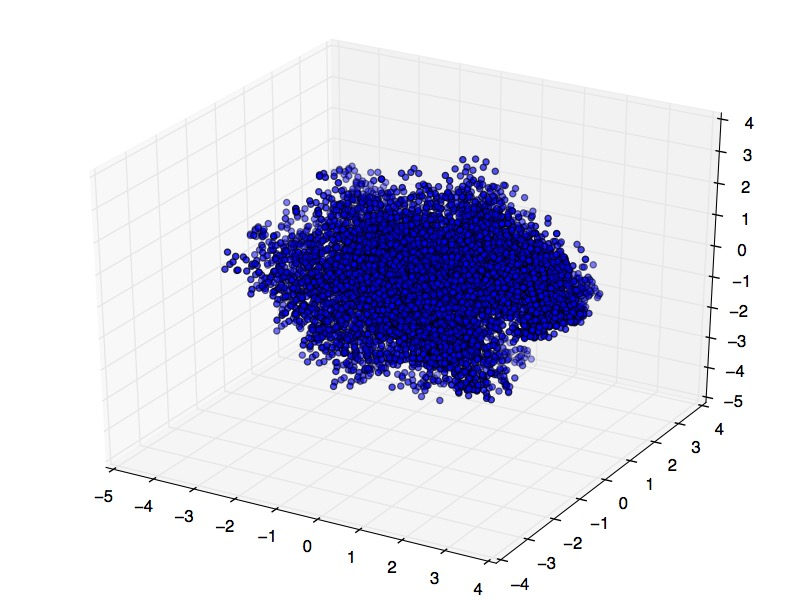
\includegraphics[width=0.5\textwidth]{../img/mappings_get10000_occ100_cos.jpg}
    \textbf{Mappings A:} $\spadesuit\clubsuit\blacksquare$
    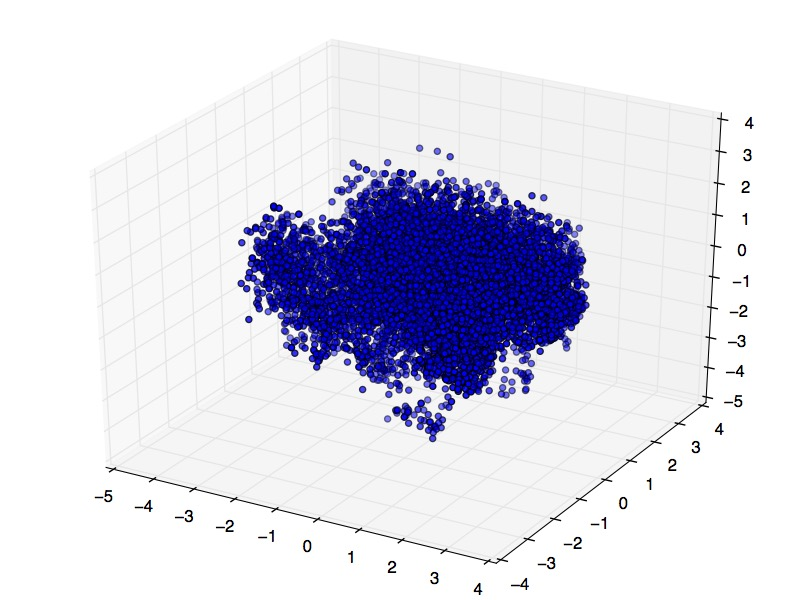
\includegraphics[width=0.5\textwidth]{../img/mappings_get10000_occ100_eucl.jpg}
    \textbf{Mappings C:} $\spadesuit\clubsuit\varheart$

    \columnbreak

    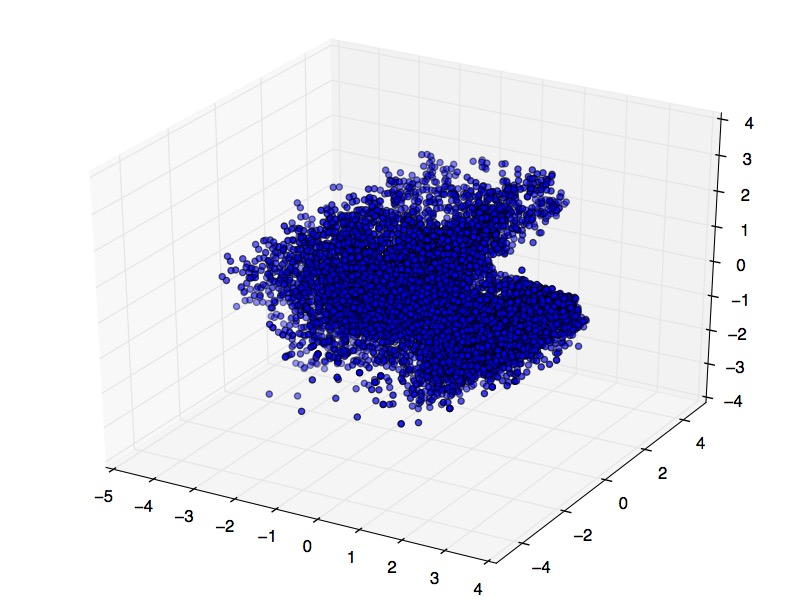
\includegraphics[width=0.5\textwidth]{../img/mappings_get10000_occ100.jpg}
    \textbf{Mappings B:} $\spadesuit\clubsuit$
    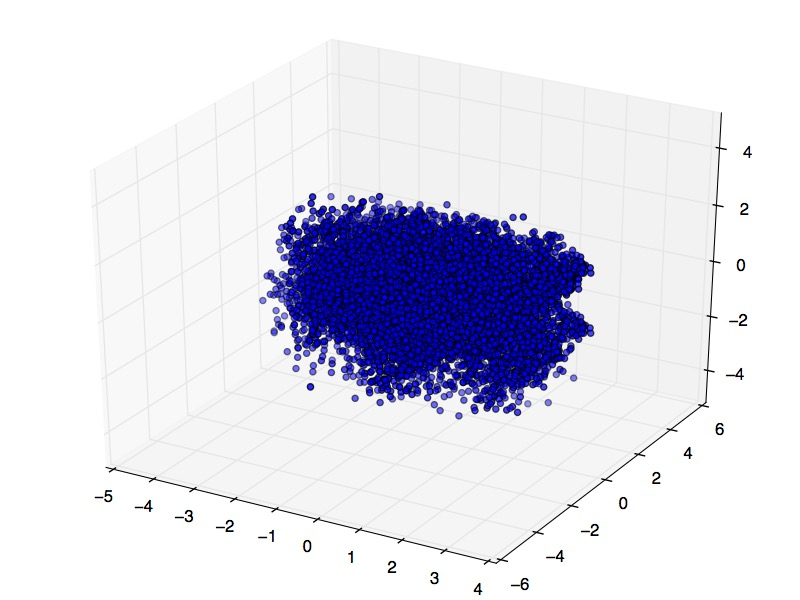
\includegraphics[width=0.5\textwidth]{../img/mappings10000_occ.jpg}
    \textbf{Mappings D:} $\spadesuit\bigstar$
  \end{multicols}

  \flushleft
  \fbox{
  \parbox{\textwidth}{
  \textbf{Feature-Legende}
  \begin{multicols}{2}
  \begin{itemize}
    \item[$\spadesuit$] $\vec{v}(t_2) - \vec{v}(t_1)$
    \item[$\bigstar$] $\Lambda(t_1, t_2) \geq 1$
    \item[$\clubsuit$] $\Lambda(t_1, t_2) \geq 100$
  \end{itemize}
  \columnbreak
  \begin{itemize}
    \item[$\blacksquare$] $cos(\vec{v}(t_2), \vec{v}(t_1))$
    \item[$\varheart$] $\parallel \vec{v}(t_2) - \vec{v}(t_1) \parallel$
  \end{itemize}
\end{multicols}
}}
  \caption[Dreidimensionale Projektionen einiger durch das Mappingverfahren resultierender Vektorräume]{Dreidimensionale
   Projektionen einiger durch das Mappingverfahren resultierender Vektorräume. Jeweils dargestellt: 10000 Vektoren.
   Symbole zeigen die jeweils genutzten Feature an. \label{fig:proj_map}}
\end{figure}

\end{itemize}

\subsection{Ansatz}

Das Fehlschlagen des Vorgehens kann auch auf einer theoretischen Ebene festgestellt werden: Das Ziel bestand darin, Wissen
über Relationen zwischen Wortpaaren zu extrahieren. Um dieses Wissen gewissermaßen ``freilegen'', muss es aber auf eine
Art und Weise innerhalb der Daten ``kodiert'' sein, wenn auch versteckt (so wie die semantische Ähnlichkeit zwischen Wörtern
durch die räumliche Nähe ihrer Vektoren und deren Dimension kodiert ist).\\
Wie beim Aufzeigen des Trugschlusses am Ende von \ref{sec:zwi-dis-data} gezeigt wurde, sind semantische Relationen nicht eindeutig
innerhalb der Daten aufzuzeigen bzw. nur dann, wenn bereits vorher bruchstückhaftes Wissen darüber vorliegt. Ohne
dieses Vorwissen sind richtige von nur scheinbaren Relationen nicht zu trennen.

% Chapter 8

\chapter{Experiment $\mathcal{C}$: Relationsvorhersage mit Wortkontextvektoren} % Main chapter title

\label{Chapter8} % For referencing the chapter elsewhere, use \ref{Chapter1}

%----------------------------------------------------------------------------------------

In diesem Kapitel soll versucht werden, die Methodik des Rausch-konstrastierenden Lernen aus Kapitel \ref{Chapter6}
auf die Wortvektoren (vgl. Kapitel \ref{Chapter5}) anzuwenden und nur die Relationsvektoren zu lernen. Zu diesem Zweck
wird eine Untermenge von FB15k, die Tripel enthält, deren Kopf- und Fußentität jeweils als Wortvektorrepräsentation vorliegen.
Schlußendlich werden die Ergebnisse evaluiert und diskutiert.

\section{Datenerzeugung}

Zu Trainingszwecken wird eine Untermenge aus FB15k bzw. GER14k gebildet. Da
die Vektorrepräsentationen für die Entitäten nicht von Grund auf erstellt sorden mit
\verb|word2vec| trainierte Vektoren verwendert werden, können nur solche Worte in dem
neuen Trainingsset vorhanden sein, zu denen ebensolche Wortvektoren auch vorliegen.
Dies ist leider nur für einen gerinen Teil der Fall, wie in Abbildung \ref{fig:we4k} zu
erkennen ist.

\begin{figure}[h]
  \centering
  \begin{changemargin}{0cm}{0cm}
  \resizebox{\textwidth}{!}) & 14.334 & (\textcolor{BrickRed}{$\downarrow$-4,12 \%}) & 1.236 & (\textcolor{BrickRed}{$\downarrow$-8,1 \%}) \\
    WE4k & 50.518 & (\textcolor{BrickRed}{$\downarrow$-91,47 \%}) & 3.623 & (\textcolor{BrickRed}{$\downarrow$-74,72 \%}) & 749 & (\textcolor{BrickRed}{$\downarrow$-39,40 \%}) \\
  \end{tabular}%
  }
\end{changemargin}
  \caption[Daten des neuen Relationsdatensets im Vergleich zu \textsc{FB15k} und \textsc{GER14k}]{Daten des neuen Sets WE4k im Vergleich mit
  FB15k und GER14k. Aufgelistet ist die Anzahl der Tripel (Datensätze), Entitäts- und Relationstypen und die Veränderung
  der Anzahlen in Prozent im Vergleich zu FB15k in Klammern.\label{fig:we4k}}
\end{figure}

Dies ist dadurch zu erklären, dass in der Quelle der Originaldaten, nämlich Freebase,
sehr viele sehr seltene Entitäten vertreten sind. Die vielen Freiwilligen, die über die
Jahre dazu beigetragen haben, die Wissensdatenbank weiter zu vervollständigen, haben dabei auch
viele unbekanntere Filme, Personen etc. hinzugefügt, die in einem Korpus eher selten zu finden sind.\\

Da die resultierende Menge an Tripeln gerundet ungefähr viertausend einzigartig Entitäten enthält, die auch als
Wortvektorrepräsentation (\emph{word embeddings}) vorliegen, wird dieses Datenset WE4k genannt.

\section{Training}

Das Training der Relationsvektoren findet in einer sehr zu der in Kapitel \ref{Chapter6} beschrieben Methode sehr
ähnlichen Art und Weise wie in Kapitel \ref{Chapter6} statt: Es wird zuerst eine Menge korrumpierter Tripel erstellt, bei denen entweder
die Kopf- oder Fußentität ersetzt wurde.
Mithilfe der ursprünglichen Tripel wird eine Menge aus Tripelpaaren erstellt, von denen der korrumpierte Teil jeweils
zufällig aus $S'$ ausgewählt wird. Auch die Verlustfunktion gestaltet sich prinzipiell gleich.\\

Der einzige Unterschied besteht in der Implementation des Algorithmus: So wird wird wegen der geringeren Menge an
Daten darauf verzichtet, für jede Trainingsanzahl eine feste Anzahl von Tripelpaaren zufällig auszuwählen.
Stattdessen richtet sich die Größe von $S_{batch}$ nach folgender Formel:

\begin{equation}
  S_{batch} \leftarrow sample(S^*, \floor*{\frac{|S^*|}{10}}+1)\footnote{Die Addtion von 1 dient dazu, bei weniger
  von 10 Tripeln für eine Relation wenigstens mit einem Tripel zu trainieren. Der Rest ist eine Heuristik.}
\end{equation}

\section{Evaluation}

Die Evaluation fand auf diesselbe Art und Weise wie im Abschnitt \ref{sec:transe-eval} statt. So wurde wieder untersucht,
inwiefern die Relationsvektoren und die Vektorrepräsentationen der Entitäten dazu genutzt werden können, ein Relationstripel
durch ``Raten'' zu vervollständigen und gemessen, welcher Rang der richtigen Antwort zugewiesen wurde und in wieivel Prozent
diese unter den Top Zehn anzutreffen war.

\begin{figure}[h]
  \centering
  \begin{tabular}{r||c|c}
    \textsc{Datenset} & \textsc{Gemittelter Rang} & \textsc{Hits@10} \\
     \hline
     WE4k & 1122,03 & 5,67 \\
     FB15k & \textbf{197,02} & \textbf{48,79} \\
     GER14k & 222,05 & 41,83 \\
  \end{tabular}
  \caption[Resultate auf mit Wordvektoren auf \textsc{WE3k}]{\label{fig:eval-we4k}}
\end{figure}

Im Blick auf Abbildung \ref{fig:eval-we4k} zeigt ein ziemlich ernüchterndes Fazit auf. So schnitt die Variante
mit Wortvektoren aus \verb|word2vec| und seperat trainierten Relationsrepräsentationen ($\rightarrow$ WE4k) im Bezug auf
den gemittelten Rang mehr als fünf Mal so schlecht und im Bezug auf die Hits\@10 mehr als acht Mal so schlecht ab.\\
Die möglichen Gründe für das weite Verfehlen guter Ergebnisse werden nun in \ref{sec:we4k-zwifa} diskutiert.

\section{Zwischenfazit}\label{sec:we4k-zwifa}

Um die Diskrepanz zwischen den Ergebnissen mit gemeinsam trainierten Repräsentationen für Entitäten und Relation im Vergleich
zu denen mit auf dem Korpus trainierten Entitäsvektoren zu erklären, sollte Unterschiedlichkeit der Ansätze hervorgehoben
werden.\\
Im ersten Fall werden wie erwähnt alle zu eine Relation betreffende Repräsentationsvektoren gemeinsam trainiert; es ist
also davon auszugehen, dass diese bestmöglichst angepasst sind, um $|h + r - t|$ für alle $h, t$ zu minimieren.\\
Dies kann im zweiten Fall nicht unbedingt gewährleistet werden: Da $h$ und $t$ im Vornherein schon feststehen und nicht
an $r$ angepasst werden (sondern genau umkehrt $r$ an $h$ und $t$ angepasst wird), kann der minimale Wert der Verlustfunktion
unter Umständen nur schwer erlangt werden.\\
Als eine weitere Begründung ist anzuführen, dass a) WE4k auf deutlich kleineren Datenmengen arbeitet (weshalb maschinelle
Lernverfahren unter umständen gar keine Lösung finden können, die gut auf ungesehene Beispiele generalisiert) und b)
Wortvektoren von sehr speziellen Entitäten enthält, die in \emph{Freebase} als Knoten existieren, u. U. aber sehr selten
im Korpus auftauchen. Da die Beschaffenheit der korpusbasierten Repräsentationen vor allem von Kookkurrenzen mit anderen
Begriffen abhängt, bedeutet eine niedrige Termfrequenz vor allem weniger aussagekräftige Wortvektoren, worunter die
Ergebnisse in der Konsequenz zu leiden haben.\\
Zuletzt sollte mit in Betracht gezogen werden, dass die trainierten Relationen sehr feingliedrig sind. Im Gegensatz zu
anderen Forschungsarbeiten, die mit grobaufgelösten Beziehungen wie ``Cause-Effect'' oder ``Entitiy-Origin''
(\cite{hendrickx2009semeval}) arbeiten, können dadurch am größere Datenmengen zugreifen und bessere Ergebnisse auf
ungesehenen Beispielen erziehlen.

% Chapter 9

\chapter{Fazit} % Main chapter title

\label{Chapter9} % For referencing the chapter elsewhere, use \ref{Chapter1}

%----------------------------------------------------------------------------------------

\begin{itquote}
  ``Mit dem Wissen wächst der Zweifel.''
  \flushright
  \textsc{Johann Wolfgang von Goethe}
\end{itquote}

\section{Zusammenfassung}

In dieser Arbeit wurden verschiedene Möglichkeiten präsentiert, Wissen aus Wissensdatenbanken durch kontinuierliche Vektorrepräsentationen
darzustellen und zu erweitern. In Kapitel \ref{Chapter6} wurden unterschiedlich komplexe Herangehensweisen vorgestellt, Repräsentationen
für Entitäten und Relationen einer solchen Datenbank gleichzeitig mithilfe von Methoden des Maschinellen Lernens zu trainieren.
Für das TransE genannte Verfahren wurden zusätzlich Ergebnisse mit einer deutschsprachigen Untermenge der Daten (\textsc{GER14k})
durchgeführt, die zwar bei der Evaluation etwas schlechter ausfielen, aber dennoch vergleichbar waren.\\

In Kapitel \ref{Chapter7} wurde ein eigener Versuch unternommen, ähnliche Ergebnisse mithilfe von Wortkontextvektoren
zu erreichen, zu deren Erstellung das Tool \verb|word2vec| verwendet wurde, welches auf großen Korpora arbeitet. Dazu
wurde der deutschsprachige Internetkorpus \textsc{DECOW14X} aufbereitet.\\
Im Folgenden wurde angestrebt, Wortvektorpaare durch ihre Differenzvektoren verschiedenen Relationen zuzuteilen. Dies schlug
jedoch fehl, da der Ansatz auf einem fehlerhaften Annahme fußte. Deshalb konnten keine evaluierbaren Ergebnisse erzeugt werden.
Eine ausführliche Diskussion darüber findet sich in \ref{sec:zwi-dis}.\\

In Kapitel \ref{Chapter8} wurde versucht, Wortkontextvektoren in das Verfahren von Kapitel \ref{Chapter6} einzubinden und nur
noch Vektorrepräsentationen für Relationen zu trainieren. Hierfür wurde ebenfalls ein Datenset namens \textsc{WE4k}
erzeugt. Wegen der Datenknappheit und anderen in \ref{sec:we4k-zwifa} diskutierten Gründen konnten hierbei keine vergleichbaren Ergebnisse
erlangt werden. Dennoch konnten einige Erkenntnisse über Wortkontextvektoren im Speziellen und Vektorrepräsentationen
im Allgemeinen daraus gezogen werden, die im nächsten Abschnitt reflektiert werden.

\section{Diskussion}

Die Implikationen der in dieser Arbeit gewonnenen Erkenntnisse sollten mit Bedacht diskutiert werden. Das Fehlschlagen
eines Ansatzes auf der Basis von Wortkontextvektoren heißt im Umkehrschluss nicht, dass alle Vorstöße in dieser
Richtung zum Scheitern verurteilt sind (im Gegenteil soll darauf in \ref{sec:fazit-ausblick} eingegangen werden).\\
Es scheint jedoch unbestreitbar leichter, Repräsentationen gleich im Kontext der Struktur einer Wissensdatenbank als im
Kontext eines großen Korpus zu trainieren, da diese so von Anfang an auf für Wissensbasen wichtige Eigenschaften getrimmt werden
(nämlich die Beziehung zu anderen Relevanten Entitäten). Jedoch erfordern solche Repräsentationen bereits viele
vorstrukturierte Datensätze, die von Menschen erstellt werden müssen.\\

Das Fehlschlagen des vorgestellten Ansatzes in Kapitel \ref{Chapter7} scheint vor allem auf einen Fehler in der
Grundannahme und die schlechte Skalierbarkeit zurückzuführen. Um Letzteres zu verhindern, könnten in zukünftigen Ansätzen
weitere Informationsquellen hinzugezogen werden, um ``sinnvolle'' von ``sinnlosen'' Wortpaaren zu trennen. Da davon
auszugehen ist, dass in der Menge aller Möglichen Wortpaare nur ein sehr kleiner Prozentsatz tatsächlich Sinn ergeben
dürfte, sollte dieses Vorgehen die totale Rechenzeit signifikaten verringern.\\
Der der Hypothese zugrunde liegende logische Fehler scheint im Nachhinein offensichtlich. Dieser war aber schwer
vorherzusehen, nachdem in vielen anderen Arbeiten die semantischen Eigenschaften von arithmetischen Rechnungen mit
Wortvektoren so stark hervorgehoben wurden. Zudem wird dieser Aspekt immer nur anhand von in einer offensichtlichen
Beziehung zueinander stehenden Wortpaaren illustriert. Dadurch fiel dieses Versäumnis erst auf, als es aus zeitlichen Gründen
nicht mehr möglich war, im Rahmen dieser Abschlussarbeit andere Verfahren zu testen und zudem Versuche, auf Basis der
vorliegenden Daten diesen Fehler zu korrigieren fehlgeschlagen waren.

\section{Ausblick}\label{sec:fazit-ausblick}

Der vorliegende Ansatz bietet vielerlei Möglichkeiten zur Verbesserung. Im Folgenden sollen einige davon skizziert werden:\\
Zuallererst erscheint es sinnvoll, das Konzept von einem unüberwachten zu einem überwachten Ansatz zu ändern, also eine
maschinellen Lernmethode mit Daten zu versorgen, denen bereits eine Klasse zugewiesen wurde. Beispielsweise könnten eine
sog. \emph{Support Vector Machine} (SVM) oder ein anderer Lernalgorithmus ein zu einer bestimmten Relation gehöriges Wortpaar
als Eingabe nehmen, um anhand dessen zu lernen zu unterscheiden, welche Differenzvektoren für eine spezifische Relationsart
charakteristisch sind. Sollte es bei einem unüberwachten Ansatz bleiben, sollten zusätzliche Informationen einer anderen Domäne
den Daten angefügt werden.\\
Innerhalb des gesamten Forschungsbereichs des maschinellen Lernens ergeben sich so verschiedenste Möglichkeiten,
sei es mit verschiedenen Features oder Algorithmen, z.B. SVMs mit Kerneln oder Neuronalen Netzwerken. Es könnte für jede
Relation eine Klasse (plus ggf. eine Klasse für Wortpaare ohne Relation) definiert werden, denen später unklassifizierte
Wortpaare zugeordnet werden.\\

Die auf dem Korpus erstellten Wortvektoren sind ein sehr aktuelles Forschungsthema. Verschiedene Ansätze wurden
präsentiert, diese weiter zu verbessern, beispielsweise auf Depenzgrammatik basierende Repräsentationen von (\cite{levy2014dependency}),
oder die als \emph{GloVe} bekanntgewordenen globalen Wortvektoren von (\cite{pennington2014glove}).
Es wäre interessant herauszufinden, inwiefern sich diese auf die Performanz eines Systems zur Relationsvorhersage
auswirken.\\

Zudem sollte sich auf eher grober aufgelöste Relationen wie in (\cite{hendrickx2009semeval}) fokussiert werden, da dies im Bezug
auf zweierlei Probleme Abhilfe verschaffen dürfte: Weil diese sich auf weniger spezielle Entitäten beziehen, ist gewährleistet,
dass die dazugehörigen Wortkontextvektoren qualitativ besser sind. Außerdem ist es in diesem Fall wahrscheinlicher, dass
sich ebenjene Relationen als Differenzvektor identifizieren lassen als wesentlich seltenere und spezielle Relationen wie
in \textsc{FB14k}.\\
Das daraus gewonnene Ergebnisse selbst in dieser Auflösungsebene hilfreich sind, wird in der Einleitung von (\cite{hendrickx2009semeval})
dargestellt:

\begin{itquote}
    ``The automatic recognition of semantic relations has many applications, such as information extraction,
    document summarization, machine translation, or construction of thesauri and semantic networks[,] [...]
    word sense disambiguation, language modeling, para-phrasing, and recognizing textual entailment.''
\end{itquote}

Abschließend bleibt festzustellen, dass Wortkontextvektoren nur eine von vielen verschiedenen Arten von kontinuierlichen
Wortvektorrepräsentationen sind, die in ihren Eigenschaft zwar beim Lösen vieler Probleme der maschinellen Sprachverarbeiten
neue Ansätze geliefert haben, aber auch nicht für jede Problemstellung als Werkzeug nützlich erscheinen.\\
Stattdessen sollten im Vornherein immer genau die Anforderungen und die Vor- und Nachteile verschiedenster Repräsentationen
gegeneinander abgewogen werden.\\

Der Wert dieser Arbeit besteht unter Anderem demnach darin, Grenzen der Wortkontextvektoren aufgezeigt zu haben, die sich abseits
des berühmten Beispiels

\begin{quote}
  $\vec{v}(King) - \vec{v}(Man) + \vec{v}(Woman) \approx \vec{v}(Queen)$
\end{quote}

in der Begeisterung über ebendiese Eigenschaft nur schwer erkennen lassen.

% Chapter 10

\chapter{Fazit} % Main chapter title

\label{Chapter10} % For referencing the chapter elsewhere, use \ref{Chapter1}

%----------------------------------------------------------------------------------------

\section{Fazit}
Bla

% Chapter 11

\chapter{Ausblick} % Main chapter title

\label{Chapter11} % For referencing the chapter elsewhere, use \ref{Chapter1}

%----------------------------------------------------------------------------------------

\section{Ausblick}
Bla


%----------------------------------------------------------------------------------------
%	THESIS CONTENT - APPENDICES
%----------------------------------------------------------------------------------------

\appendix % Cue to tell LaTeX that the following "chapters" are Appendices

% Include the appendices of the thesis as separate files from the Appendices folder
% Uncomment the lines as you write the Appendices

% Appendix A

\chapter{Übersicht über Trainingsparameter der Wortkontextvektoren} % Main appendix title

\label{AppendixA} % For referencing this appendix elsewhere, use \ref{AppendixA}

\begin{figure}[h]
\centering
\begin{tabular}{c||l|l|l|l|l}
  \textsc{Nr.} & \textsc{Korpus} & \textsc{Prep} & \textsc{Training} & \textsc{NEG} & \textsc{Sampling} \\
  \hline \hline
  \Romannum{1} & Decow & - & Skip-gram & 5 & $1^-5$ \\
  \hline
  \Romannum{2} & Decow & - & Skip-gram & 5 & $1^-4$ \\
  \hline
  \Romannum{3} & Decow & - & Skip-gram & 5 & $1^-3$ \\
  \hline
  \Romannum{4} & Decow & - & Skip-gram & 5 & $0,01$ \\
  \hline
  \Romannum{5} & Decow & - & Skip-gram & 5 & $0,1$ \\
  \hline
  \Romannum{6} & Decow & - & Skip-gram & 5 & $1$ \\
  \hline
  \Romannum{7} & Decow & - & CBOW & 5 & $1^-5$ \\
  \hline
  \Romannum{8} & Decow & - & CBOW & 5 & $1^-4$ \\
  \hline
  \Romannum{9} & Decow & - & CBOW & 5 & $1^-3$ \\
  \hline
  \Romannum{10} & Decow & - & CBOW & 5 & $0,01$ \\
  \hline
  \Romannum{11} & Decow & - & CBOW & 5 & $0,1$ \\
  \hline
  \Romannum{12} & Decow & - & CBOW & 5 & $1$ \\
  \hline
  \Romannum{13} & Decow & Lemmatisiert & Skip-gram & 5 & $1^-5$ \\
  \hline
  \Romannum{14} & Decow & Lemmatisiert & Skip-gram & 5 & $1^-4$ \\
  \hline
  \Romannum{15} & Decow & Lemmatisiert & Skip-gram & 5 & $1^-3$ \\
  \hline
  \Romannum{16} & Decow & Lemmatisiert & Skip-gram & 5 & $0,01$ \\
  \hline
  \Romannum{17} & Decow & Lemmatisiert & Skip-gram & 5 & $0,1$ \\
  \hline
  \Romannum{18} & Decow & Lemmatisiert & Skip-gram & 5 & $1$ \\
  \hline
  \Romannum{19} & Decow & Lemmatisiert & CBOW & 5 & $1^-5$ \\
  \hline
  \Romannum{20} & Decow & Lemmatisiert & CBOW & 5 & $1^-4$ \\
  \hline
  \Romannum{21} & Decow & Lemmatisiert & CBOW & 5 & $1^-3$ \\
  \hline
  \Romannum{22} & Decow & Lemmatisiert & CBOW & 5 & $0,01$ \\
  \hline
  \Romannum{23} & Decow & Lemmatisiert & CBOW & 5 & $0,1$ \\
  \hline
  \Romannum{24} & Decow & Lemmatisiert & CBOW & 5 & $1$ \\
\end{tabular}
\caption[Trainingsparameter der Wortkontextvektoren]{Quelle und Trainingsparameter für verschiedenen Sets von Wortkontextvektoren.
\textsc{Prep} = Aufbereitung des Korpus vor dem Training; \textsc{Training} = Verwendete Trainingsmethode; \textsc{NEG} = Anzahl der
Negativbeispiele beim Training; \textsc{Sampling} = Ausmaß des Downsamplings häufiger Wörter.}
\end{figure}

% Appendix Template

\chapter{Evaluationen der Wortvektoren} % Main appendix title
%\addtolength{\topmargin}{-0.875in}

\label{AppendixB} % Change X to a consecutive letter; for referencing this appendix elsewhere, use \ref{AppendixX}

Evaluationsergebnisse bei Wortähnlichkeit und Analogien für die verschiedenen Datensets.
Für weitere Informationen über die Grundlage der Vektoren siehe Appendix \ref{AppendixA}.
Wörter außerhalb des Vokabulars wurden entweder als Fehler gerechnet, oder
werden, falls anders nicht möglich, als Zahl im Index in runden Klammern angegeben.

\vspace{1cm}

  \centering
  \rotatebox{-90}{%
  \small
  \resizebox{1.2525\columnwidth}{!}{%
  \begin{tabular}{l||c|c|c|c||c|c}
     & \multicolumn{4}{c}{Wortähnlichkeit ($\rho \in [-1, 1]$)} & \multicolumn{2}{c}{Analogien (in \%)} \\
    Datenset & \textsc{Wortpaare65} & \textsc{Wortpaare222} & \textsc{Wortpaare350} & \textsc{Schm280} & \textsc{Google} & \textsc{SemRel} \\
    \hline \hline
    Mark I & -0,8096 & & -0,7302$_{(13)}$ & & 44,56 & \\
    \hline
    Mark II & -0,7856 & & -0,7156$_{(13)}$ & & 40,37 &  \\
    \hline
    Mark III & -0,7718 & & -0,6886$_{(13)}$ & & 27,42 & 35,11 \\
    \hline
    Mark IV & -0,7681 & & -0,6834$_{(13)}$ & & 25,48 & 32,03 \\
    \hline
    Mark V &  -0,7725 & & -0,6738$_{(13)}$ & & 25,54 &  \\
    \hline
    Mark VI & -0,7697 & & -0,6784$_{(13)}$ & & 25,52 &  \\
    \hline
    Mark VII & -0,7255 & & -0,6924$_{(13)}$ & & 30,60 & 1,50  \\
    \hline
    Mark VIII & -0,6149 & & -0,6530$_{(13)}$ & & 26,98 &  \\
    \hline
    Mark IX & -0,6784 & & -0,6090$_{(13)}$ & & 22,26 & 1,62 \\
    \hline
    Mark X & -0,5949 & & -0,5791$_{(13)}$ & & 19,22 & 1,22 \\
    \hline
    Mark XI & -0,5890 & & -0,5700$_{(13)}$ & & 18,60 & 1,38  \\
    \hline
    Mark XII & -0,5874 & & -0,5706$_{(13)}$ & & 8,62 &  \\
    \hline
    Mark XIII & \textbf{-0,8247$_{(1)}$} & & \textbf{-0,7494$_{(132)}$} & & 15,51 & 3,01 \\
    \hline
    Mark XIV & -0,8106$_{(1)}$ & & -0,7362$_{(132)}$ & & 14,51 & 2,56 \\
    \hline
    Mark XV & -0,7786$_{(1)}$ & & -0,7136$_{(132)}$ & & 13,15 & 2,44 \\
    \hline
    Mark XVI & -0,7576$_{(1)}$ & & -0,6990$_{(132)}$ & & 11,76 & 2,56 \\
    \hline
    Mark XVII & -0,7578$_{(1)}$ & & -0,6986$_{(132)}$ & & 11,41 & 2,80 \\
    \hline
    Mark XVIII & -0,7551$_{(1)}$  & & -0,6981$_{(132)}$ & 11,38 & & 3,01 \\
    \hline
    Mark XIX & -0,7589$_{(1)}$  & & -0,7476$_{(132)}$ & & & 2,23 \\
    \hline
    Mark XX & -0,7519$_{(1)}$ & & -0,7239$_{(132)}$ & & & 2,15 \\
    \hline
    Mark XXI & -0,7188$_{(1)}$ & & -0,6875$_{(132)}$ & & 9,68 & 1,75 \\
    \hline
    Mark XXII & -0,6926$_{(1)}$ & & -0,6429$_{(132)}$ & & & 1,71 \\
    \hline
    Mark XXIII & -0,6851$_{(1)}$ & & -0,6359$_{(132)}$ & & & 1,95 \\
    \hline
    Mark XXIV & -0,6913$_{(1)}$ & & -0,6369$_{(132)}$ & & & 2,07 \\
  \end{tabular}%
  }%
  }

  \restoregeometry

%\include{Appendices/AppendixC}

%----------------------------------------------------------------------------------------
%	BIBLIOGRAPHY
%----------------------------------------------------------------------------------------

\printbibliography[heading=bibintoc]

%----------------------------------------------------------------------------------------

\end{document}
